% Options for packages loaded elsewhere
\PassOptionsToPackage{unicode}{hyperref}
\PassOptionsToPackage{hyphens}{url}
\PassOptionsToPackage{dvipsnames,svgnames,x11names}{xcolor}
\documentclass[
  10pt,
]{article}
\usepackage{xcolor}
\usepackage[margin=1.8cm]{geometry}
\usepackage{amsmath,amssymb}
\setcounter{secnumdepth}{-\maxdimen} % remove section numbering
\usepackage{iftex}
\ifPDFTeX
  \usepackage[T1]{fontenc}
  \usepackage[utf8]{inputenc}
  \usepackage{textcomp} % provide euro and other symbols
\else % if luatex or xetex
  \usepackage{unicode-math} % this also loads fontspec
  \defaultfontfeatures{Scale=MatchLowercase}
  \defaultfontfeatures[\rmfamily]{Ligatures=TeX,Scale=1}
\fi
\usepackage{lmodern}
\ifPDFTeX\else
  % xetex/luatex font selection
\fi
% Use upquote if available, for straight quotes in verbatim environments
\IfFileExists{upquote.sty}{\usepackage{upquote}}{}
\IfFileExists{microtype.sty}{% use microtype if available
  \usepackage[]{microtype}
  \UseMicrotypeSet[protrusion]{basicmath} % disable protrusion for tt fonts
}{}
\makeatletter
\@ifundefined{KOMAClassName}{% if non-KOMA class
  \IfFileExists{parskip.sty}{%
    \usepackage{parskip}
  }{% else
    \setlength{\parindent}{0pt}
    \setlength{\parskip}{6pt plus 2pt minus 1pt}}
}{% if KOMA class
  \KOMAoptions{parskip=half}}
\makeatother
\usepackage{longtable,booktabs,array}
\newcounter{none} % for unnumbered tables
\usepackage{calc} % for calculating minipage widths
% Correct order of tables after \paragraph or \subparagraph
\usepackage{etoolbox}
\makeatletter
\patchcmd\longtable{\par}{\if@noskipsec\mbox{}\fi\par}{}{}
\makeatother
% Allow footnotes in longtable head/foot
\IfFileExists{footnotehyper.sty}{\usepackage{footnotehyper}}{\usepackage{footnote}}
\makesavenoteenv{longtable}
\usepackage{graphicx}
\makeatletter
\newsavebox\pandoc@box
\newcommand*\pandocbounded[1]{% scales image to fit in text height/width
  \sbox\pandoc@box{#1}%
  \Gscale@div\@tempa{\textheight}{\dimexpr\ht\pandoc@box+\dp\pandoc@box\relax}%
  \Gscale@div\@tempb{\linewidth}{\wd\pandoc@box}%
  \ifdim\@tempb\p@<\@tempa\p@\let\@tempa\@tempb\fi% select the smaller of both
  \ifdim\@tempa\p@<\p@\scalebox{\@tempa}{\usebox\pandoc@box}%
  \else\usebox{\pandoc@box}%
  \fi%
}
% Set default figure placement to htbp
\def\fps@figure{htbp}
\makeatother
\setlength{\emergencystretch}{3em} % prevent overfull lines
\providecommand{\tightlist}{%
  \setlength{\itemsep}{0pt}\setlength{\parskip}{0pt}}

\usepackage{etoolbox}
\AtBeginEnvironment{longtable}{\scriptsize}
\usepackage{float}
\let\origfigure\figure
\let\endorigfigure\endfigure
\renewenvironment{figure}[1][2] {\expandafter\origfigure\expandafter[H]} {\endorigfigure}
\usepackage{bookmark}
\IfFileExists{xurl.sty}{\usepackage{xurl}}{} % add URL line breaks if available
\urlstyle{same}
\hypersetup{
  pdftitle={qrig: a verified implementation of the control equations of One rig to control them all --- consolidated results},
  colorlinks=true,
  linkcolor={Maroon},
  filecolor={Maroon},
  citecolor={Blue},
  urlcolor={Blue},
  pdfcreator={LaTeX via pandoc}}

\title{qrig: a verified implementation of the control equations of
\emph{One rig to control them all} --- consolidated results}
\usepackage{etoolbox}
\makeatletter
\providecommand{\subtitle}[1]{% add subtitle to \maketitle
  \apptocmd{\@title}{\par {\large #1 \par}}{}{}
}
\makeatother
\subtitle{All-to-all noise study, resource, time, fault-tolerance and
robustness metrics}
\author{}
\date{generated by python/benchmarks/make\_report.py}

\begin{document}
\maketitle

{
\setcounter{tocdepth}{3}
\tableofcontents
}
This document collects every result obtained with the \texttt{qrig}
package so far. It is generated from the JSON result files by
\texttt{python/benchmarks/make\_report.py}; the PDF and the Markdown
file have the same content. All numbers are \textbf{classical
simulations} (Qiskit 2.5.2, Qiskit Aer 0.17.2, qrig 1.1.0, Python
3.11.14, 8 CPU cores). No real quantum hardware was used. The Lean
proofs cover the optimiser core, not the measurements reported here.

\textbf{Key findings} (details and exceptions in Sections 4--9; summary
repeated in Section 11):

\begin{itemize}
\tightlist
\item
  \textbf{Correctness}: every rewrite is proved sound in Lean; all 130
  circuits checked exactly were identical after qrig; no circuit in any
  run was found non-equivalent.
\item
  \textbf{Do no harm}: CX model: fewer 2q gates on 21, equal on 109,
  more on 0 of 130 circuits; CZ model: fewer 2q gates on 20, equal on
  108, more on 2 of 130 circuits; RXX model: fewer 2q gates on 22, equal
  on 108, more on 0 of 130 circuits.
\item
  \textbf{Where it helps}: qrig lowers the CZ-model two-qubit count in 4
  application categories (arithmetic, control patterns, data loading \&
  block encoding, search \& oracles): circuits with multi-controlled
  gates next to each other or conjugated by NOT gates --- Grover and SAT
  oracles, membership oracles, QROM / table lookup, LCU SELECT oracles,
  multiplexers, the MQT multipliers, compute/uncompute blocks. On
  circuits without such structure (QFT, QPE, VQE/QAOA ans\"{a}tze, GHZ,
  W-state, Trotter circuits, swap test) it changes nothing and costs a
  few milliseconds.
\item
  \textbf{Noise}: over the 66 simulated (circuit, target) pairs that
  qrig changes, the fidelity is higher with qrig in 62 and lower in 4
  (grover 7 on CZ model: output close to fully mixed for both, F \ensuremath{\approx} 2.1 \ensuremath{\times}
  2\textsuperscript{\ensuremath{-}}\textsuperscript{\ensuremath{n}} with n = 7; grover 10 on RXX model: output close to fully mixed
  for both, F \ensuremath{\approx} 1.0 \ensuremath{\times} 2\textsuperscript{\ensuremath{-}}\textsuperscript{\ensuremath{n}} with n = 10; hrs\_cumulative\_multiplier 5 on
  CZ model: qrig + Qiskit ends with more two-qubit gates, 122 \ensuremath{\rightarrow} 128;
  hrs\_cumulative\_multiplier 9 on CZ model: qrig + Qiskit ends with
  more two-qubit gates, 484 \ensuremath{\rightarrow} 494). Where the fidelity rises, the gain
  holds from \ensuremath{\tfrac{1}{4}}\ensuremath{\times} to 4\ensuremath{\times} today's error rates and under gate-only, idle-only
  and coherent noise (Section 8).
\item
  \textbf{Other compilers}: Qiskit O3: qrig + Qiskit O3 has fewer 2q
  gates on 21, equal on 109, more on 0 of 130 circuits, total 29398 \ensuremath{\rightarrow}
  21896 (-25.5 \%); TKET: qrig + TKET has fewer 2q gates on 17, equal on
  112, more on 1 of 130 circuits, total 31933 \ensuremath{\rightarrow} 26305 (-17.6 \%);
  BQSKit: qrig + BQSKit has fewer 2q gates on 24, equal on 69, more on 0
  of 93 circuits, total 10697 \ensuremath{\rightarrow} 7423 (-30.6 \%). The benefit is
  therefore not specific to Qiskit. TKET alone already reaches qrig's
  saving on the MQT Grover and multiplier circuits; on data loading
  (QROM, LCU SELECT, multiplexers), membership oracles and the control
  patterns, qrig lowers the count in front of all three compilers
  (Section 9).
\item
  \textbf{Time}: the qrig pass costs milliseconds; the compiled circuits
  are shorter on the device and need fewer shots.
\item
  \textbf{Fault tolerance}: T-count is mixed (Section 7).
\end{itemize}

\section{1. Answers to the questions behind this
study}\label{answers-to-the-questions-behind-this-study}

\textbf{Is robustness a valid metric?} Yes, if it is defined precisely.
In this study \emph{robustness} means: does the benefit of adding qrig
survive when the conditions change? We measure three versions of it: (i)
across compiler randomness (10 transpiler seeds per circuit and target),
(ii) across noise strength (all error rates of the CZ model scaled from
\ensuremath{\tfrac{1}{4}}\ensuremath{\times} to 4\ensuremath{\times}), and (iii) across noise type (stochastic gate errors only,
idle decoherence only, coherent over-rotations, coherent + idle). A pass
whose gains vanish or reverse under one of these is fragile. Section 8
shows that, wherever qrig lowers the two-qubit count, the gain survives
all of these changes; the exceptions are listed there.

\textbf{Is equivalence a robustness metric?} No.~Equivalence (the
optimised circuit implements exactly the same unitary) is a
\textbf{correctness} property, and for qrig it is a \emph{guarantee},
not a statistic: every rewrite rule is proved sound in Lean 4
(\texttt{peephole\_sound}), and the executable core is compiled from
that Lean code to C. We still check it empirically (exact unitary
comparison and ideal-output comparison for every circuit, Section 3)
because the Python \ensuremath{\leftrightarrow} Qiskit bridge is not proved. Correctness should be
reported as its own column (``verified / checked''), next to the
performance metrics, not as one of them.

\textbf{Which metrics show that qrig is useful?} We report six families,
all with all-to-all connectivity so that hardware topology cannot bias
the result:

{\def\LTcaptype{none} % do not increment counter
\begin{longtable}[]{@{}
  >{\raggedright\arraybackslash}p{(\linewidth - 4\tabcolsep) * \real{0.3333}}
  >{\raggedright\arraybackslash}p{(\linewidth - 4\tabcolsep) * \real{0.3333}}
  >{\raggedright\arraybackslash}p{(\linewidth - 4\tabcolsep) * \real{0.3333}}@{}}
\toprule\noalign{}
\begin{minipage}[b]{\linewidth}\raggedright
family
\end{minipage} & \begin{minipage}[b]{\linewidth}\raggedright
metric(s)
\end{minipage} & \begin{minipage}[b]{\linewidth}\raggedright
why it matters
\end{minipage} \\
\midrule\noalign{}
\endhead
\bottomrule\noalign{}
\endlastfoot
correctness & proved rewrite soundness; exact unitary check; ideal
outputs agree & an optimiser that may change the circuit is unusable \\
resources & two-qubit gate count, depth, two-qubit depth & two-qubit
gates dominate error and time on every platform \\
noise & state fidelity F, task success P, estimated success probability
ESP & what a user actually gets out of a noisy device \\
time & qrig pass time, Qiskit compile time, scheduled execution time,
shots needed \ensuremath{\propto} 1/F\textsuperscript{2} & cost of using qrig vs time saved on the device \\
fault tolerance & T-count and arbitrary rotations after Clifford+T+Rz
compilation & cost on future error-corrected machines \\
robustness & seed spread, noise-strength sweep, noise-type sweep &
whether the gains are an artefact of one setting \\
\end{longtable}
}

\textbf{Is the all-to-all experiment complete?} The earlier all-to-all
experiment covered 17 circuits that were \emph{selected because qrig
reduced their gate count}. That is enough to show the effect exists, but
it is a biased sample. This study extends it to \textbf{130 circuits}:
every unitary MQT Bench benchmark at up to three sizes (87 circuits, not
hand-picked), 37 application kernels written the textbook way
(SAT-oracle Grover, membership oracles, QROM table lookup, LCU SELECT
oracles, comparators, adders, Shor's modular adder, Hamming weight,
state preparation, swap test, Ising Trotter steps, \ldots), and the 6
control-pattern circuits of the earlier study; on three all-to-all
targets, with all metric families above. Circuits up to 10 qubits are
simulated exactly with density matrices; the earlier 12- and 16-qubit
multiplier runs are included in Section 10. Section 9 repeats the
comparison with two other compilers, TKET and BQSKit.

\section{2. What qrig adds to the original
paper}\label{what-qrig-adds-to-the-original-paper}

The paper \emph{One rig to control them all} gives a sound and complete
equational theory for quantum circuits with controlled gates (control
equations (a)--(h), Figure 1). It does not give an implementation, an
optimisation algorithm, or a measurement of their effect on noisy
hardware. qrig contributes:

\begin{enumerate}
\def\labelenumi{\arabic{enumi}.}
\tightlist
\item
  \textbf{A verified implementation.} The circuit language, its
  semantics, exact arithmetic in \ensuremath{\mathbb{Q}}(\ensuremath{\omega}), an exact equivalence checker,
  Gray-code permutation synthesis and a rewrite optimiser are written in
  Lean 4; the eight control equations and the soundness of every rewrite
  the optimiser performs are proved (no \texttt{sorry}, standard axioms
  only). The C code that runs is generated by the Lean compiler from
  this code.
\item
  \textbf{An optimisation algorithm built from the equations} (the paper
  has none): fusion/cancellation (a, b), complementarity C\textsuperscript{0}(f)\ensuremath{\cdot}C\textsuperscript{1}(f) = f
  (e), commutation (f) and diagonal commutation, and colour change ---
  pushing NOT gates through controls (d) --- applied to whole Qiskit
  DAGs within a 128-gate window.
\item
  \textbf{A usable package}: \texttt{import\ qrig}, a Qiskit transpiler
  pass (\texttt{QrigControlEquations}) that can be put in front of any
  Qiskit pipeline, conversion to/from Qiskit, and a test-suite (265
  tests) against Qiskit's simulators.
\item
  \textbf{The empirical study in this document}: which real circuits
  benefit, by how much in gates, fidelity and time, and how robust the
  effect is.
\end{enumerate}

Equivalence of every optimised circuit is a theorem, so improvements
never cost correctness. The study below shows what they buy.

\section{3. Set-up}\label{set-up}

\textbf{Pipelines.} \emph{Qiskit alone} = Qiskit's preset pass manager
at optimisation level 3 (its strongest). \emph{qrig + Qiskit} =
\texttt{qrig.dag.optimize\_circuit} first, then the same level-3 pass
manager. For each circuit, target and pipeline we compile with 10
transpiler seeds and keep the compilation with the highest estimated
success probability (what a user would do); the spread over seeds is
reported in Section 6.

\textbf{Targets.} All three targets are all-to-all; they differ in
native two-qubit gate (CX, CZ, RXX) and noise parameters. The CZ model
uses the median FakeTorino calibration (an IBM Heron-generation snapshot
shipped with Qiskit); the RXX model uses assumed values. Only the
calibration numbers are borrowed: the CZ model is not a model of that
device, which is not all-to-all and whose readout error and crosstalk
are omitted here. Below, the targets are called the CX, CZ and RXX
models.

{\def\LTcaptype{none} % do not increment counter
\begin{longtable}[]{@{}
  >{\raggedright\arraybackslash}p{(\linewidth - 4\tabcolsep) * \real{0.3333}}
  >{\raggedright\arraybackslash}p{(\linewidth - 4\tabcolsep) * \real{0.3333}}
  >{\raggedright\arraybackslash}p{(\linewidth - 4\tabcolsep) * \real{0.3333}}@{}}
\toprule\noalign{}
\begin{minipage}[b]{\linewidth}\raggedright
target
\end{minipage} & \begin{minipage}[b]{\linewidth}\raggedright
native gates
\end{minipage} & \begin{minipage}[b]{\linewidth}\raggedright
noise model
\end{minipage} \\
\midrule\noalign{}
\endhead
\bottomrule\noalign{}
\endlastfoot
CX model & cx, rz, sx, x & p2 = 0.3\%, p1 = 0.03\%, no idle noise \\
CZ model & cz, rz, sx, x & median FakeTorino calibration: cz error
0.419\%, 1q error 0.0271\%, cz 0.068 \ensuremath{\mu}s, 1q 0.032 \ensuremath{\mu}s, T1 185 \ensuremath{\mu}s, T2
138.2 \ensuremath{\mu}s; idle relaxation in an ALAP schedule \\
RXX model & rxx, rz, sx, x & assumed round numbers (not a vendor
calibration): rxx error 0.5\%, 1q error 0.03\%, rxx 600 \ensuremath{\mu}s, 1q 100 \ensuremath{\mu}s,
T1 1e+08 \ensuremath{\mu}s, T2 1e+06 \ensuremath{\mu}s; idle relaxation \\
\end{longtable}
}

\textbf{Circuits.}

{\def\LTcaptype{none} % do not increment counter
\begin{longtable}[]{@{}
  >{\raggedright\arraybackslash}p{(\linewidth - 4\tabcolsep) * \real{0.3333}}
  >{\raggedright\arraybackslash}p{(\linewidth - 4\tabcolsep) * \real{0.3333}}
  >{\raggedright\arraybackslash}p{(\linewidth - 4\tabcolsep) * \real{0.3333}}@{}}
\toprule\noalign{}
\begin{minipage}[b]{\linewidth}\raggedright
suite
\end{minipage} & \begin{minipage}[b]{\linewidth}\raggedright
circuits
\end{minipage} & \begin{minipage}[b]{\linewidth}\raggedright
families (qubit counts)
\end{minipage} \\
\midrule\noalign{}
\endhead
\bottomrule\noalign{}
\endlastfoot
MQT Bench (neutral suite) & 87 & ae (4, 7, 10); bmw\_quark\_cardinality
(4, 7, 10); bmw\_quark\_copula (4, 8, 10); bv (4, 7, 10);
cdkm\_ripple\_carry\_adder (4, 8, 10); dj (4, 7, 10); draper\_qft\_adder
(4, 8, 10); full\_adder (4, 8, 10); ghz (4, 7, 10); graphstate (4, 7,
10); grover (4, 7, 10); half\_adder (5, 7, 9); hhl (4, 7, 10);
hrs\_cumulative\_multiplier (5, 9); modular\_adder (4, 8, 10);
multiplier (4, 8); qaoa (4, 7, 10); qft (4, 7, 10); qftentangled (4, 7,
10); qnn (4, 7, 10); qpeexact (4, 7, 10); qpeinexact (4, 7, 10); qwalk
(4, 7, 10); randomcircuit (4, 7, 10); rg\_qft\_multiplier (4, 8);
vbe\_ripple\_carry\_adder (4, 7, 10); vqe\_real\_amp (4, 7, 10);
vqe\_su2 (4, 7, 10); vqe\_two\_local (4, 7, 10); wstate (4, 7, 10) \\
application kernels & 37 & comparator (6, 8, 10); grover\_sat (7, 9,
10); hamming\_weight (5, 8, 10); incrementer (4, 6, 8); ising\_trotter
(6, 10); lcu\_select (5, 6, 8); lib\_grover (4, 5, 6);
membership\_oracle (5, 7); poly\_rotation (4, 6); qrom (5, 6, 8, 8);
shor\_modadd (7, 8); state\_prep (3, 5); swap\_test (5, 7, 9);
weighted\_adder (9, 10) \\
control-pattern circuits & 6 & C3(H);C3(V);C3(V\^{}-1);C3(H) (4); C3(T)
(4); compute/uncompute U;U\^{}-1 (4); multiplexer (4, 5, 6) \\
\end{longtable}
}

The MQT suite contains every unitary benchmark of MQT Bench at the
algorithm level (dynamic circuits with mid-circuit measurement, and
benchmarks with no instance in the size range, are excluded). Sizes are
the smallest, middle and largest admissible size between 4 and 10
qubits. The application kernels are written the way a Qiskit user writes
them (library objects or the textbook construction); their source is
\texttt{python/benchmarks/app\_circuits.py}. The control-pattern
circuits contain exactly the patterns the control equations target and
are reported separately so that they do not inflate the averages.

\textbf{Metrics.} F = state fidelity \ensuremath{\langle}\ensuremath{\psi}\textbar \ensuremath{\rho}\textbar \ensuremath{\psi}\ensuremath{\rangle} averaged
over 3 random product input states; P = Hellinger fidelity of the output
distribution for one classical input (the success probability when the
answer is deterministic); \emph{error removed} = 1 \ensuremath{-} (1 \ensuremath{-} F\_qrig)/(1 \ensuremath{-}
F\_Qiskit); \emph{ratio} = F\_qrig/F\_Qiskit; ESP = \ensuremath{\prod}(1 \ensuremath{-} e\_gate). When
noise scales a measured signal by F, the shots needed for a fixed
precision scale like 1/F\textsuperscript{2}, so the \emph{shot saving} is
(F\_qrig/F\_Qiskit)\textsuperscript{2}. Duration = length of the ALAP-scheduled compiled
circuit.

\subsection{3.1 Correctness checks (all
circuits)}\label{correctness-checks-all-circuits}

\begin{itemize}
\tightlist
\item
  qrig rewrote 88 of the 130 circuits (at least one rule applied).
\item
  Exact unitary comparison, qrig output vs input circuit: 130 of 130
  circuits identical up to 10\textsuperscript{\ensuremath{-}}\textsuperscript{8} in every matrix entry (not up to global
  phase --- exactly).
\item
  Ideal (noise-free) outputs of the two compiled circuits agree in 390
  of 390 (circuit, target) pairs, and agree with the statevector of the
  original benchmark in 390 of 390.
\item
  Earlier MQT pipeline run (74 circuits up to 128 qubits): MQT QCEC
  proved the qrig output equivalent for 72 circuits; the rest timed out;
  none was found non-equivalent.
\end{itemize}

\subsection{3.2 What is proved in Lean about the kernels and the
metrics}\label{what-is-proved-in-lean-about-the-kernels-and-the-metrics}

Besides the soundness of every qrig rewrite, \texttt{QrigProofs/Study/}
proves what several application kernels compute and the properties of
the metrics this report relies on (no \texttt{sorry}, standard axioms
only):

{\def\LTcaptype{none} % do not increment counter
\begin{longtable}[]{@{}
  >{\raggedright\arraybackslash}p{(\linewidth - 4\tabcolsep) * \real{0.3333}}
  >{\raggedright\arraybackslash}p{(\linewidth - 4\tabcolsep) * \real{0.3333}}
  >{\raggedright\arraybackslash}p{(\linewidth - 4\tabcolsep) * \real{0.3333}}@{}}
\toprule\noalign{}
\begin{minipage}[b]{\linewidth}\raggedright
file
\end{minipage} & \begin{minipage}[b]{\linewidth}\raggedright
theorems
\end{minipage} & \begin{minipage}[b]{\linewidth}\raggedright
statement
\end{minipage} \\
\midrule\noalign{}
\endhead
\bottomrule\noalign{}
\endlastfoot
\texttt{Reversible.lean} & \texttt{incrementer\_spec},
\texttt{hamming\_weight\_correct}, \texttt{memberOracle\_spec},
\texttt{qrom\_spec} & incrementer adds 1 mod 2\textsuperscript{\ensuremath{n}}; the Hamming-weight
counter ends with the popcount; the membership oracle flips its target
iff the input is in the set; QROM XORs table{[}address{]} into the data
register \\
\texttt{Reversible.lean} & \texttt{run\_xconj} & colour change (d) on
basis states: NOT gates around a block flip the polarity of the controls
they touch (the rewrite qrig applies to these kernels) \\
\texttt{Draper.lean} & \texttt{phiAdd\_correct},
\texttt{phiAddOld\_wrong} & the phase angles of the Draper adder in
\texttt{shor\_modadd} map QFT\textbar x\ensuremath{\rangle} to QFT\textbar(x+a) mod 2\textsuperscript{\ensuremath{n}}\ensuremath{\rangle}
under Qiskit's \texttt{QFTGate} convention; the angle formula used
before a fix during the study does not \\
\texttt{Metrics.lean} & \texttt{esp\_sublist\_le},
\texttt{espUniform\_robust}, \texttt{espUniform\_tradeoff\_not\_robust}
& removing gates never lowers ESP; no more 1q and no more 2q gates \ensuremath{\Rightarrow} ESP
at least as high at every noise scale; with a 1q/2q trade-off the ESP
comparison can flip \\
\texttt{Metrics.lean} & \texttt{shotsNeeded\_div},
\texttt{geomean\_le\_one}, \texttt{geomean\_lt\_one} & shot saving =
(F\_qrig/F\_Qiskit)\textsuperscript{2}; if no circuit gets worse the per-circuit
geometric-mean ratio is \ensuremath{\leq} 1, and \textless{} 1 once one circuit
improves \\
\end{longtable}
}

The kernel theorems are about a Lean gate-list model written to mirror
\texttt{python/benchmarks/app\_circuits.py};
\texttt{python/tests/test\_kernels.py} runs the actual Qiskit circuits
on every basis state and checks them against the same specifications.
The simulated numbers themselves are not checked in Lean.

\section{4. Resources: two-qubit gates and
depth}\label{resources-two-qubit-gates-and-depth}

\begin{figure}
\centering
\pandocbounded{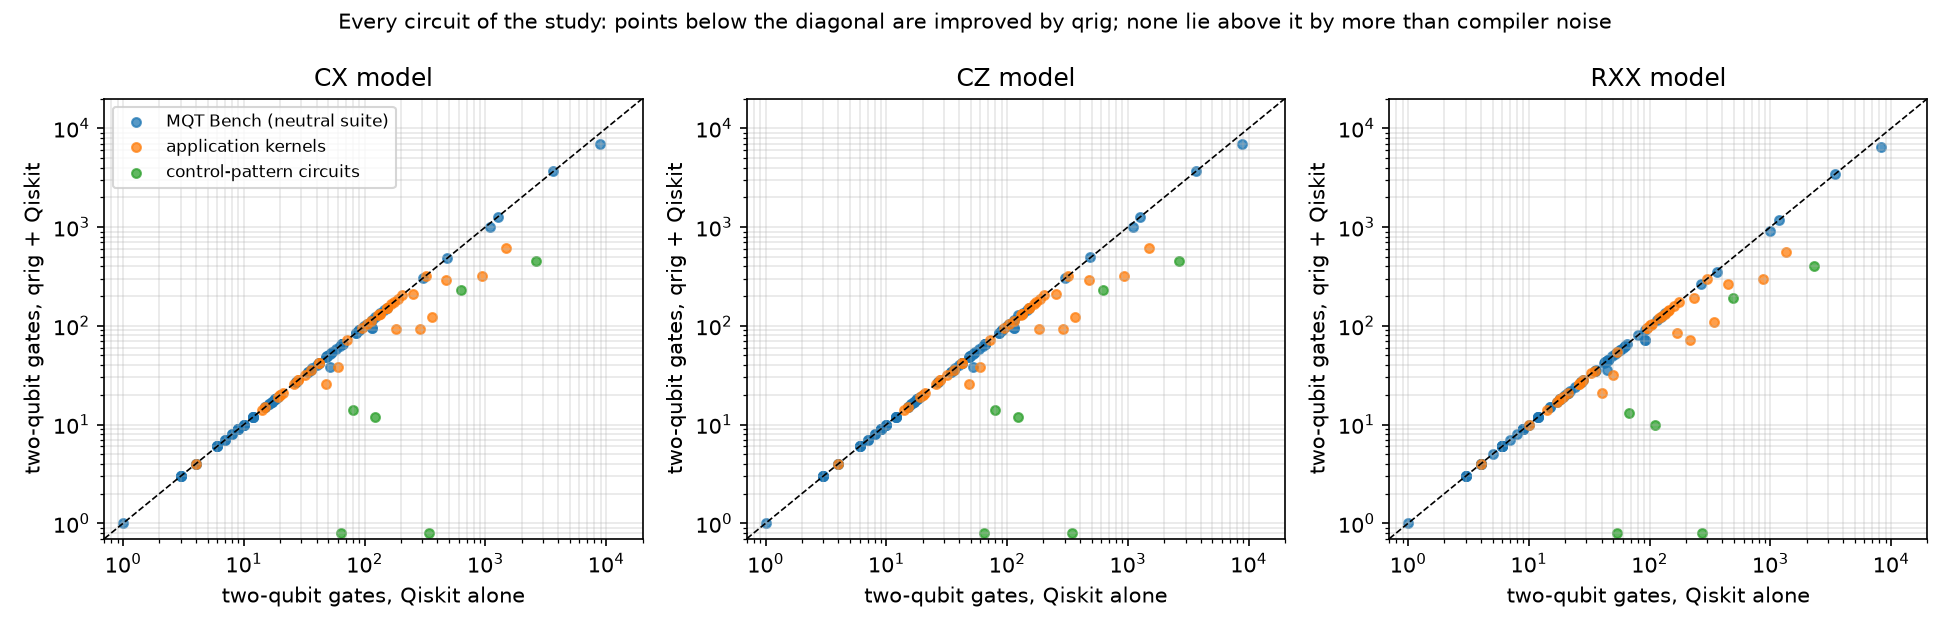
\includegraphics[keepaspectratio,alt={Two-qubit gate count of every circuit, Qiskit alone vs qrig + Qiskit, on the three all-to-all targets.}]{figures/fig1_twoq_all_circuits.png}}
\caption{Two-qubit gate count of every circuit, Qiskit alone vs qrig +
Qiskit, on the three all-to-all targets.}
\end{figure}

{\def\LTcaptype{none} % do not increment counter
\begin{longtable}[]{@{}
  >{\raggedright\arraybackslash}p{(\linewidth - 12\tabcolsep) * \real{0.1429}}
  >{\raggedright\arraybackslash}p{(\linewidth - 12\tabcolsep) * \real{0.1429}}
  >{\raggedright\arraybackslash}p{(\linewidth - 12\tabcolsep) * \real{0.1429}}
  >{\raggedright\arraybackslash}p{(\linewidth - 12\tabcolsep) * \real{0.1429}}
  >{\raggedright\arraybackslash}p{(\linewidth - 12\tabcolsep) * \real{0.1429}}
  >{\raggedright\arraybackslash}p{(\linewidth - 12\tabcolsep) * \real{0.1429}}
  >{\raggedright\arraybackslash}p{(\linewidth - 12\tabcolsep) * \real{0.1429}}@{}}
\toprule\noalign{}
\begin{minipage}[b]{\linewidth}\raggedright
suite
\end{minipage} & \begin{minipage}[b]{\linewidth}\raggedright
target
\end{minipage} & \begin{minipage}[b]{\linewidth}\raggedright
fewer 2q
\end{minipage} & \begin{minipage}[b]{\linewidth}\raggedright
equal
\end{minipage} & \begin{minipage}[b]{\linewidth}\raggedright
more 2q
\end{minipage} & \begin{minipage}[b]{\linewidth}\raggedright
total 2q gates
\end{minipage} & \begin{minipage}[b]{\linewidth}\raggedright
change
\end{minipage} \\
\midrule\noalign{}
\endhead
\bottomrule\noalign{}
\endlastfoot
MQT Bench (neutral suite) & CX model & 6 & 81 & 0 & 18961 \ensuremath{\rightarrow} 16907 &
-10.8 \% \\
MQT Bench (neutral suite) & CZ model & 5 & 80 & 2 & 18961 \ensuremath{\rightarrow} 16925 &
-10.7 \% \\
MQT Bench (neutral suite) & RXX model & 7 & 80 & 0 & 16854 \ensuremath{\rightarrow} 14995 &
-11.0 \% \\
application kernels & CX model & 9 & 28 & 0 & 6578 \ensuremath{\rightarrow} 4279 & -34.9 \% \\
application kernels & CZ model & 9 & 28 & 0 & 6578 \ensuremath{\rightarrow} 4279 & -34.9 \% \\
application kernels & RXX model & 9 & 28 & 0 & 5858 \ensuremath{\rightarrow} 3779 & -35.5 \% \\
control-pattern circuits & CX model & 6 & 0 & 0 & 3859 \ensuremath{\rightarrow} 710 & -81.6
\% \\
control-pattern circuits & CZ model & 6 & 0 & 0 & 3859 \ensuremath{\rightarrow} 710 & -81.6
\% \\
control-pattern circuits & RXX model & 6 & 0 & 0 & 3302 \ensuremath{\rightarrow} 614 & -81.4
\% \\
\textbf{all} & CX model & 21 & 109 & 0 & 29398 \ensuremath{\rightarrow} 21896 & -25.5 \% \\
\textbf{all} & CZ model & 20 & 108 & 2 & 29398 \ensuremath{\rightarrow} 21914 & -25.5 \% \\
\textbf{all} & RXX model & 22 & 108 & 0 & 26014 \ensuremath{\rightarrow} 19388 & -25.5 \% \\
\end{longtable}
}

\emph{fewer/equal/more}: number of circuits where qrig + Qiskit has
fewer / the same / more two-qubit gates than Qiskit alone (best seed of
each).

Circuits whose two-qubit count changes on at least one target:

{\def\LTcaptype{none} % do not increment counter
\begin{longtable}[]{@{}
  >{\raggedright\arraybackslash}p{(\linewidth - 12\tabcolsep) * \real{0.1429}}
  >{\raggedright\arraybackslash}p{(\linewidth - 12\tabcolsep) * \real{0.1429}}
  >{\raggedright\arraybackslash}p{(\linewidth - 12\tabcolsep) * \real{0.1429}}
  >{\raggedright\arraybackslash}p{(\linewidth - 12\tabcolsep) * \real{0.1429}}
  >{\raggedright\arraybackslash}p{(\linewidth - 12\tabcolsep) * \real{0.1429}}
  >{\raggedright\arraybackslash}p{(\linewidth - 12\tabcolsep) * \real{0.1429}}
  >{\raggedright\arraybackslash}p{(\linewidth - 12\tabcolsep) * \real{0.1429}}@{}}
\toprule\noalign{}
\begin{minipage}[b]{\linewidth}\raggedright
circuit
\end{minipage} & \begin{minipage}[b]{\linewidth}\raggedright
qubits
\end{minipage} & \begin{minipage}[b]{\linewidth}\raggedright
2q (CX)
\end{minipage} & \begin{minipage}[b]{\linewidth}\raggedright
2q (CZ)
\end{minipage} & \begin{minipage}[b]{\linewidth}\raggedright
2q (RXX)
\end{minipage} & \begin{minipage}[b]{\linewidth}\raggedright
depth (CZ)
\end{minipage} & \begin{minipage}[b]{\linewidth}\raggedright
rules applied
\end{minipage} \\
\midrule\noalign{}
\endhead
\bottomrule\noalign{}
\endlastfoot
grover 4 & 4 & 52 \ensuremath{\rightarrow} 38 & 52 \ensuremath{\rightarrow} 38 & 44 \ensuremath{\rightarrow} 36 & 186 \ensuremath{\rightarrow} 148 & xconj 4 \\
grover 7 & 7 & 1092 \ensuremath{\rightarrow} 996 & 1092 \ensuremath{\rightarrow} 996 & 990 \ensuremath{\rightarrow} 918 & 3463 \ensuremath{\rightarrow} 3298 & xconj
30 \\
grover 10 & 10 & 8874 \ensuremath{\rightarrow} 6970 & 8874 \ensuremath{\rightarrow} 6970 & 8211 \ensuremath{\rightarrow} 6477 & 28913 \ensuremath{\rightarrow} 22799
& xconj 136 \\
hrs\_cumulative\_multiplier 5 & 5 & 122 \ensuremath{\rightarrow} 122 & 122 \ensuremath{\rightarrow} 128 & 91 \ensuremath{\rightarrow} 90 &
438 \ensuremath{\rightarrow} 458 & fuse 1, cancel 1 \\
hrs\_cumulative\_multiplier 9 & 9 & 484 \ensuremath{\rightarrow} 482 & 484 \ensuremath{\rightarrow} 494 & 358 \ensuremath{\rightarrow} 352 &
1743 \ensuremath{\rightarrow} 1772 & fuse 4, cancel 4 \\
multiplier 8 & 8 & 115 \ensuremath{\rightarrow} 96 & 115 \ensuremath{\rightarrow} 96 & 91 \ensuremath{\rightarrow} 72 & 272 \ensuremath{\rightarrow} 233 & idRem
4 \\
rg\_qft\_multiplier 8 & 8 & 115 \ensuremath{\rightarrow} 96 & 115 \ensuremath{\rightarrow} 96 & 91 \ensuremath{\rightarrow} 72 & 272 \ensuremath{\rightarrow} 233 &
idRem 4 \\
qrom 2x3 & 5 & 48 \ensuremath{\rightarrow} 26 & 48 \ensuremath{\rightarrow} 26 & 40 \ensuremath{\rightarrow} 21 & 188 \ensuremath{\rightarrow} 100 & compl 2, xconj
4 \\
qrom 3x3 & 6 & 182 \ensuremath{\rightarrow} 92 & 182 \ensuremath{\rightarrow} 92 & 169 \ensuremath{\rightarrow} 85 & 688 \ensuremath{\rightarrow} 351 & compl 4,
xconj 12 \\
qrom 3x5 & 8 & 364 \ensuremath{\rightarrow} 122 & 364 \ensuremath{\rightarrow} 122 & 338 \ensuremath{\rightarrow} 110 & 1356 \ensuremath{\rightarrow} 447 & compl
12, xconj 12 \\
qrom 4x4 & 8 & 936 \ensuremath{\rightarrow} 322 & 936 \ensuremath{\rightarrow} 322 & 864 \ensuremath{\rightarrow} 297 & 3431 \ensuremath{\rightarrow} 1185 & compl
17, xconj 32 \\
lcu\_select 2x3 & 5 & 60 \ensuremath{\rightarrow} 38 & 60 \ensuremath{\rightarrow} 38 & 50 \ensuremath{\rightarrow} 32 & 239 \ensuremath{\rightarrow} 145 & compl 2,
xconj 4 \\
lcu\_select 3x3 & 6 & 252 \ensuremath{\rightarrow} 208 & 252 \ensuremath{\rightarrow} 208 & 234 \ensuremath{\rightarrow} 192 & 951 \ensuremath{\rightarrow} 790 &
cancel 5, compl 2, xconj 12 \\
lcu\_select 3x5 & 8 & 476 \ensuremath{\rightarrow} 289 & 476 \ensuremath{\rightarrow} 289 & 442 \ensuremath{\rightarrow} 265 & 1781 \ensuremath{\rightarrow} 1068 &
cancel 11, compl 9, xconj 12 \\
membership\_oracle 4 & 5 & 288 \ensuremath{\rightarrow} 92 & 288 \ensuremath{\rightarrow} 92 & 216 \ensuremath{\rightarrow} 72 & 1040 \ensuremath{\rightarrow} 333 &
compl 4, xconj 19 \\
membership\_oracle 6 & 7 & 1488 \ensuremath{\rightarrow} 606 & 1488 \ensuremath{\rightarrow} 606 & 1356 \ensuremath{\rightarrow} 556 & 4320 \ensuremath{\rightarrow}
1923 & compl 5, xconj 33 \\
multiplexer (3 controls) & 4 & 122 \ensuremath{\rightarrow} 12 & 122 \ensuremath{\rightarrow} 12 & 111 \ensuremath{\rightarrow} 10 & 443 \ensuremath{\rightarrow} 49
& compl 5 \\
multiplexer (4 controls) & 5 & 624 \ensuremath{\rightarrow} 232 & 624 \ensuremath{\rightarrow} 232 & 492 \ensuremath{\rightarrow} 192 & 2061
\ensuremath{\rightarrow} 765 & compl 7 \\
multiplexer (5 controls) & 6 & 2626 \ensuremath{\rightarrow} 452 & 2626 \ensuremath{\rightarrow} 452 & 2305 \ensuremath{\rightarrow} 399 &
8085 \ensuremath{\rightarrow} 1578 & compl 20 \\
C3(T) x4 & 4 & 80 \ensuremath{\rightarrow} 14 & 80 \ensuremath{\rightarrow} 14 & 68 \ensuremath{\rightarrow} 13 & 255 \ensuremath{\rightarrow} 57 & fuse 3 \\
compute/uncompute U;U\^{}-1 & 4 & 343 \ensuremath{\rightarrow} 0 & 343 \ensuremath{\rightarrow} 0 & 272 \ensuremath{\rightarrow} 0 & 1137 \ensuremath{\rightarrow} 0
& cancel 29, xconj 1 \\
C3(H);C3(V);C3(V\^{}-1);C3(H) & 4 & 64 \ensuremath{\rightarrow} 0 & 64 \ensuremath{\rightarrow} 0 & 54 \ensuremath{\rightarrow} 0 & 227 \ensuremath{\rightarrow} 0 &
cancel 2 \\
\end{longtable}
}

Rules: \texttt{xconj} colour change (d), \texttt{compl} complementarity
(e), \texttt{cancel}/\texttt{fuse} equations (a)/(b), \texttt{idRem}
identity removal.

\subsection{4.1 Results by application
category}\label{results-by-application-category}

To show that the effect is not limited to one algorithm (e.g.~Grover),
the circuits are grouped by what they are used for. \emph{fewer/more}:
circuits with fewer / more two-qubit gates after qrig; the percentage is
the change of the category total.

{\def\LTcaptype{none} % do not increment counter
\begin{longtable}[]{@{}
  >{\raggedright\arraybackslash}p{(\linewidth - 12\tabcolsep) * \real{0.1429}}
  >{\raggedright\arraybackslash}p{(\linewidth - 12\tabcolsep) * \real{0.1429}}
  >{\raggedright\arraybackslash}p{(\linewidth - 12\tabcolsep) * \real{0.1429}}
  >{\raggedright\arraybackslash}p{(\linewidth - 12\tabcolsep) * \real{0.1429}}
  >{\raggedright\arraybackslash}p{(\linewidth - 12\tabcolsep) * \real{0.1429}}
  >{\raggedright\arraybackslash}p{(\linewidth - 12\tabcolsep) * \real{0.1429}}
  >{\raggedright\arraybackslash}p{(\linewidth - 12\tabcolsep) * \real{0.1429}}@{}}
\toprule\noalign{}
\begin{minipage}[b]{\linewidth}\raggedright
category
\end{minipage} & \begin{minipage}[b]{\linewidth}\raggedright
circuits
\end{minipage} & \begin{minipage}[b]{\linewidth}\raggedright
families
\end{minipage} & \begin{minipage}[b]{\linewidth}\raggedright
rewritten
\end{minipage} & \begin{minipage}[b]{\linewidth}\raggedright
CX target: fewer/more; total
\end{minipage} & \begin{minipage}[b]{\linewidth}\raggedright
CZ: fewer/more; total
\end{minipage} & \begin{minipage}[b]{\linewidth}\raggedright
largest CZ reduction
\end{minipage} \\
\midrule\noalign{}
\endhead
\bottomrule\noalign{}
\endlastfoot
search \& oracles & 17 & 6 & 17 & 5/0; -24.7 \% & 5/0; -24.7 \% &
membership\_oracle 4 (288 \ensuremath{\rightarrow} 92) \\
arithmetic & 37 & 14 & 25 & 3/0; -1.3 \% & 2/2; -0.7 \% & multiplier 8
(115 \ensuremath{\rightarrow} 96) \\
data loading \& block encoding & 14 & 5 & 14 & 10/0; -66.1 \% & 10/0;
-66.1 \% & multiplexer (3 controls) (122 \ensuremath{\rightarrow} 12) \\
Fourier \& phase estimation & 18 & 6 & 6 & 0/0; +0.0 \% & 0/0; +0.0 \% &
-- \\
simulation \& walks & 5 & 2 & 5 & 0/0; +0.0 \% & 0/0; +0.0 \% & -- \\
variational, ML \& finance & 21 & 7 & 12 & 0/0; +0.0 \% & 0/0; +0.0 \% &
-- \\
states \& primitives & 15 & 5 & 6 & 0/0; +0.0 \% & 0/0; +0.0 \% & -- \\
control patterns & 3 & 3 & 3 & 3/0; -97.1 \% & 3/0; -97.1 \% &
compute/uncompute U;U\^{}-1 (343 \ensuremath{\rightarrow} 0) \\
\end{longtable}
}

Outside search/oracle circuits and the control-pattern circuits, qrig
lowers the CZ-model two-qubit count on 12 of 110 circuits.

Per-circuit view (each circuit weighted equally, so a few large circuits
cannot dominate):

{\def\LTcaptype{none} % do not increment counter
\begin{longtable}[]{@{}
  >{\raggedright\arraybackslash}p{(\linewidth - 8\tabcolsep) * \real{0.2000}}
  >{\raggedright\arraybackslash}p{(\linewidth - 8\tabcolsep) * \real{0.2000}}
  >{\raggedright\arraybackslash}p{(\linewidth - 8\tabcolsep) * \real{0.2000}}
  >{\raggedright\arraybackslash}p{(\linewidth - 8\tabcolsep) * \real{0.2000}}
  >{\raggedright\arraybackslash}p{(\linewidth - 8\tabcolsep) * \real{0.2000}}@{}}
\toprule\noalign{}
\begin{minipage}[b]{\linewidth}\raggedright
target
\end{minipage} & \begin{minipage}[b]{\linewidth}\raggedright
geometric mean of 2q ratio, all circuits
\end{minipage} & \begin{minipage}[b]{\linewidth}\raggedright
geometric mean, circuits whose count changes
\end{minipage} & \begin{minipage}[b]{\linewidth}\raggedright
median reduction where it drops
\end{minipage} & \begin{minipage}[b]{\linewidth}\raggedright
largest reduction
\end{minipage} \\
\midrule\noalign{}
\endhead
\bottomrule\noalign{}
\endlastfoot
CX model & 0.893 & 0.467 & 49 \% & 100 \% \\
CZ model & 0.894 & 0.487 & 54 \% & 100 \% \\
RXX model & 0.893 & 0.486 & 49 \% & 100 \% \\
\end{longtable}
}

\section{5. Noise: fidelity of the compiled
circuits}\label{noise-fidelity-of-the-compiled-circuits}

\begin{figure}
\centering
\pandocbounded{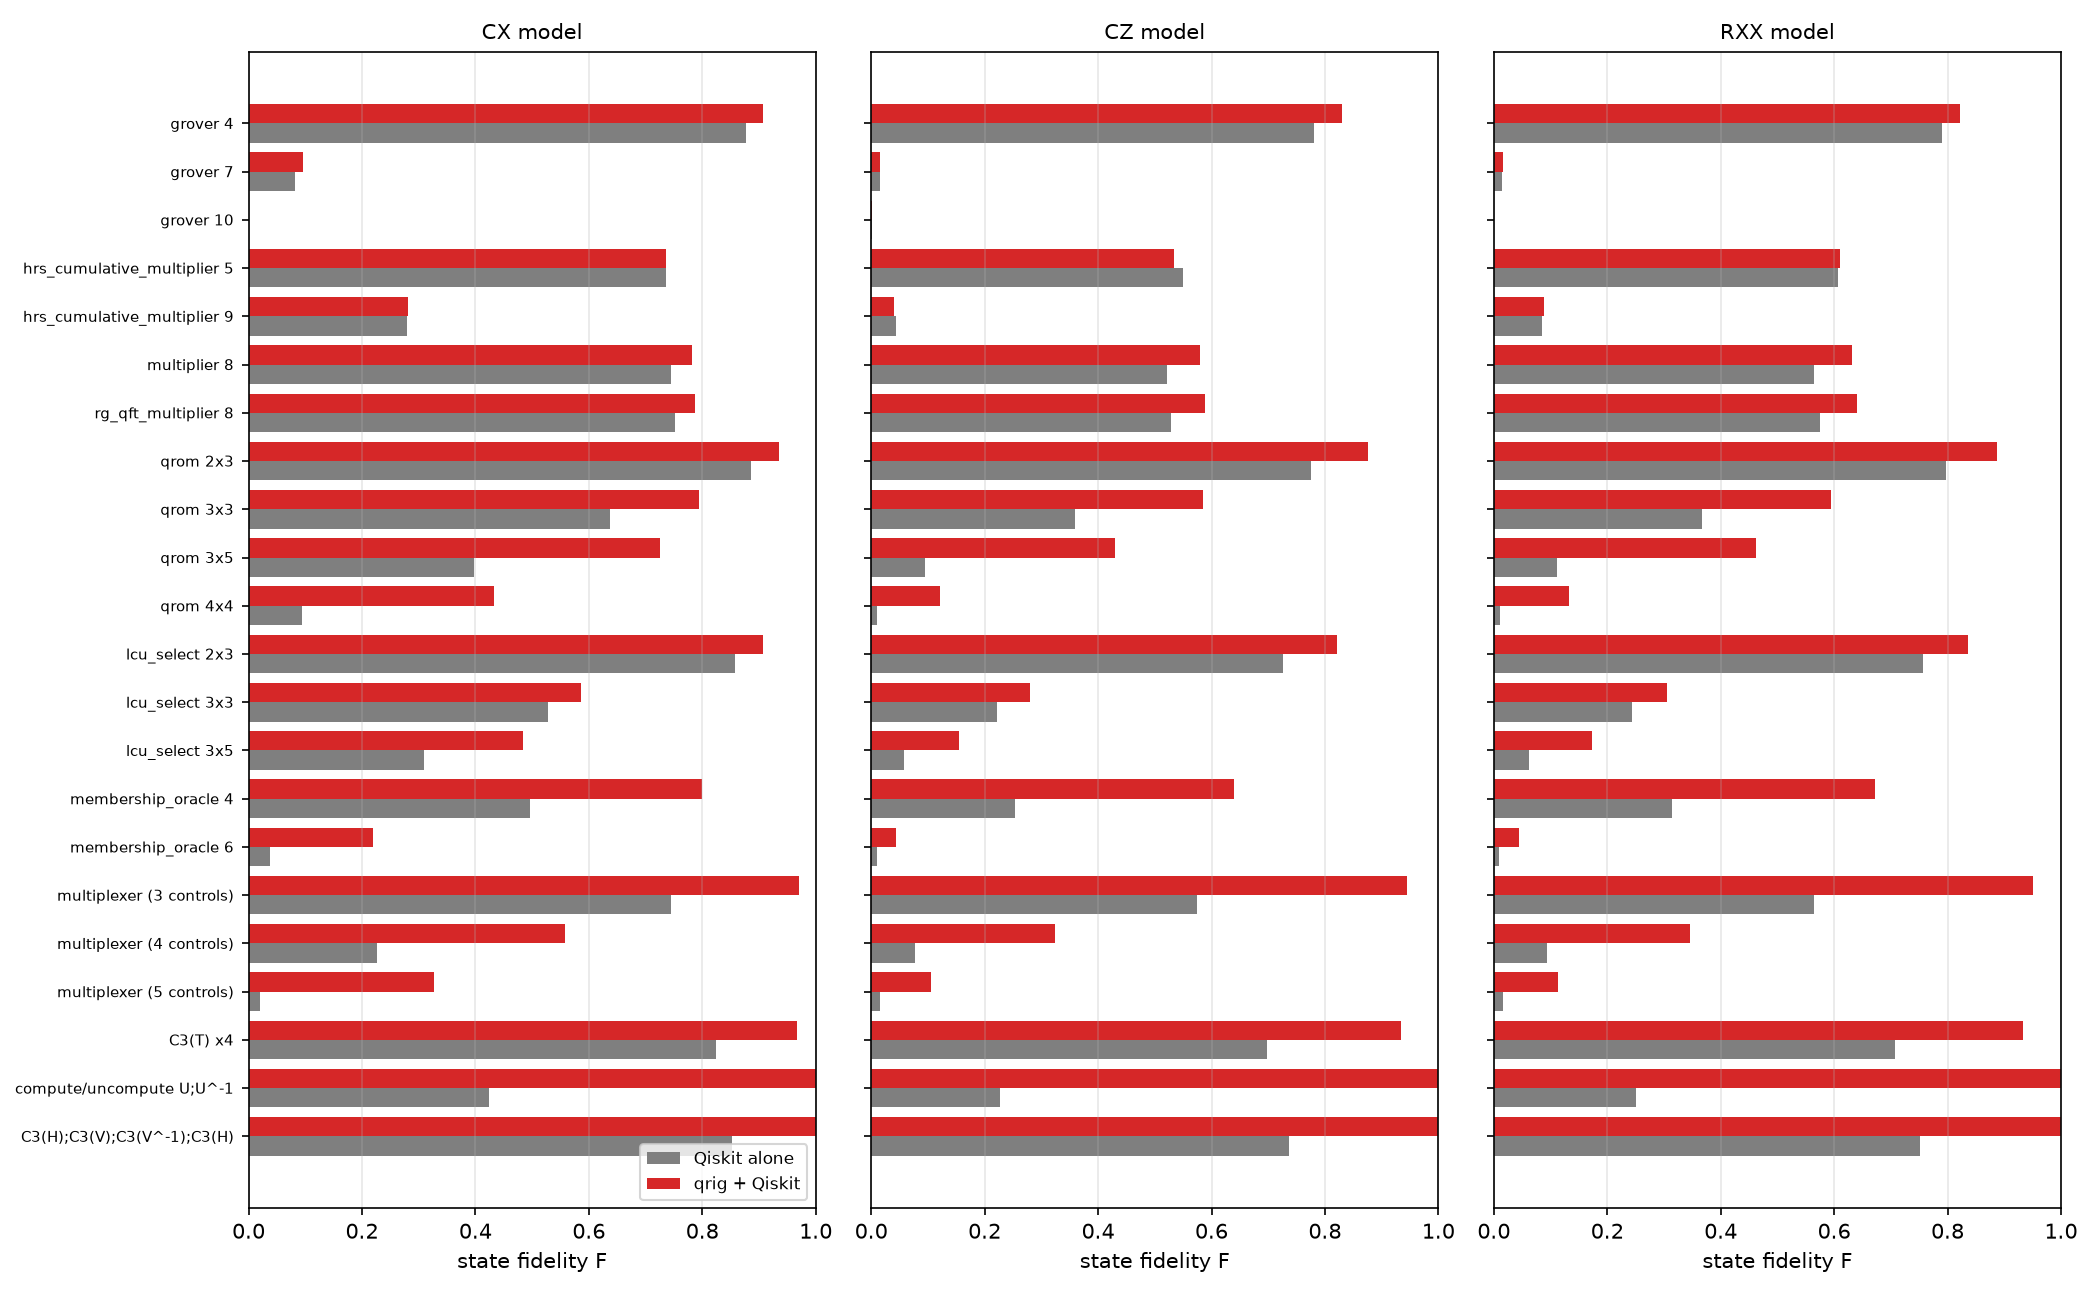
\includegraphics[keepaspectratio,alt={State fidelity with and without qrig, circuits whose gate count qrig changes.}]{figures/fig2_fidelity.png}}
\caption{State fidelity with and without qrig, circuits whose gate count
qrig changes.}
\end{figure}

{\def\LTcaptype{none} % do not increment counter
\begin{longtable}[]{@{}
  >{\raggedright\arraybackslash}p{(\linewidth - 12\tabcolsep) * \real{0.1429}}
  >{\raggedright\arraybackslash}p{(\linewidth - 12\tabcolsep) * \real{0.1429}}
  >{\raggedright\arraybackslash}p{(\linewidth - 12\tabcolsep) * \real{0.1429}}
  >{\raggedright\arraybackslash}p{(\linewidth - 12\tabcolsep) * \real{0.1429}}
  >{\raggedright\arraybackslash}p{(\linewidth - 12\tabcolsep) * \real{0.1429}}
  >{\raggedright\arraybackslash}p{(\linewidth - 12\tabcolsep) * \real{0.1429}}
  >{\raggedright\arraybackslash}p{(\linewidth - 12\tabcolsep) * \real{0.1429}}@{}}
\toprule\noalign{}
\begin{minipage}[b]{\linewidth}\raggedright
circuit
\end{minipage} & \begin{minipage}[b]{\linewidth}\raggedright
F (CX)
\end{minipage} & \begin{minipage}[b]{\linewidth}\raggedright
F (CZ)
\end{minipage} & \begin{minipage}[b]{\linewidth}\raggedright
F (RXX)
\end{minipage} & \begin{minipage}[b]{\linewidth}\raggedright
error removed (CZ)
\end{minipage} & \begin{minipage}[b]{\linewidth}\raggedright
ratio (CZ)
\end{minipage} & \begin{minipage}[b]{\linewidth}\raggedright
shot saving (CZ)
\end{minipage} \\
\midrule\noalign{}
\endhead
\bottomrule\noalign{}
\endlastfoot
grover 4 & 0.876 \ensuremath{\rightarrow} 0.906 & 0.781 \ensuremath{\rightarrow} 0.830 & 0.790 \ensuremath{\rightarrow} 0.823 & +22 \% &
\ensuremath{\times}1.06 & \ensuremath{\times}1.13 \\
grover 7 & 0.081 \ensuremath{\rightarrow} 0.096 & 0.016 \ensuremath{\rightarrow} 0.015 & 0.014 \ensuremath{\rightarrow} 0.015 (scr.) & -0 \%
& \ensuremath{\times}0.94 & \ensuremath{\times}0.88 \\
grover 10 & 1.0e-03 \ensuremath{\rightarrow} 1.0e-03 (scr.) & 9.5e-04 \ensuremath{\rightarrow} 1.0e-03 (scr.) &
9.8e-04 \ensuremath{\rightarrow} 9.8e-04 (scr.) & +0 \% & \ensuremath{\times}1.08 & -- \\
hrs\_cumulative\_multiplier 5 & 0.736 \ensuremath{\rightarrow} 0.737 & 0.549 \ensuremath{\rightarrow} 0.533 & 0.606 \ensuremath{\rightarrow}
0.610 & -3 \% & \ensuremath{\times}0.97 & \ensuremath{\times}0.94 \\
hrs\_cumulative\_multiplier 9 & 0.280 \ensuremath{\rightarrow} 0.281 & 0.044 \ensuremath{\rightarrow} 0.041 & 0.085 \ensuremath{\rightarrow}
0.088 & -0 \% & \ensuremath{\times}0.93 & \ensuremath{\times}0.86 \\
multiplier 8 & 0.745 \ensuremath{\rightarrow} 0.781 & 0.521 \ensuremath{\rightarrow} 0.580 & 0.565 \ensuremath{\rightarrow} 0.631 & +12 \% &
\ensuremath{\times}1.11 & \ensuremath{\times}1.24 \\
rg\_qft\_multiplier 8 & 0.751 \ensuremath{\rightarrow} 0.787 & 0.528 \ensuremath{\rightarrow} 0.589 & 0.575 \ensuremath{\rightarrow} 0.640 &
+13 \% & \ensuremath{\times}1.12 & \ensuremath{\times}1.25 \\
qrom 2x3 & 0.885 \ensuremath{\rightarrow} 0.935 & 0.775 \ensuremath{\rightarrow} 0.876 & 0.798 \ensuremath{\rightarrow} 0.886 & +45 \% &
\ensuremath{\times}1.13 & \ensuremath{\times}1.28 \\
qrom 3x3 & 0.638 \ensuremath{\rightarrow} 0.793 & 0.359 \ensuremath{\rightarrow} 0.584 & 0.367 \ensuremath{\rightarrow} 0.594 & +35 \% &
\ensuremath{\times}1.63 & \ensuremath{\times}2.65 \\
qrom 3x5 & 0.397 \ensuremath{\rightarrow} 0.726 & 0.096 \ensuremath{\rightarrow} 0.430 & 0.112 \ensuremath{\rightarrow} 0.462 & +37 \% &
\ensuremath{\times}4.49 & \ensuremath{\times}20.19 \\
qrom 4x4 & 0.094 \ensuremath{\rightarrow} 0.433 & 9.5e-03 \ensuremath{\rightarrow} 0.122 & 0.011 \ensuremath{\rightarrow} 0.132 & +11 \% &
\ensuremath{\times}12.78 & \ensuremath{\times}163.43 \\
lcu\_select 2x3 & 0.858 \ensuremath{\rightarrow} 0.906 & 0.727 \ensuremath{\rightarrow} 0.821 & 0.757 \ensuremath{\rightarrow} 0.836 & +34 \%
& \ensuremath{\times}1.13 & \ensuremath{\times}1.28 \\
lcu\_select 3x3 & 0.529 \ensuremath{\rightarrow} 0.587 & 0.221 \ensuremath{\rightarrow} 0.281 & 0.244 \ensuremath{\rightarrow} 0.305 & +8 \%
& \ensuremath{\times}1.27 & \ensuremath{\times}1.61 \\
lcu\_select 3x5 & 0.310 \ensuremath{\rightarrow} 0.483 & 0.057 \ensuremath{\rightarrow} 0.155 & 0.061 \ensuremath{\rightarrow} 0.173 & +10 \%
& \ensuremath{\times}2.72 & \ensuremath{\times}7.42 \\
membership\_oracle 4 & 0.497 \ensuremath{\rightarrow} 0.799 & 0.253 \ensuremath{\rightarrow} 0.640 & 0.314 \ensuremath{\rightarrow} 0.672 &
+52 \% & \ensuremath{\times}2.53 & \ensuremath{\times}6.39 \\
membership\_oracle 6 & 0.038 \ensuremath{\rightarrow} 0.219 & 0.010 \ensuremath{\rightarrow} 0.044 & 9.6e-03 \ensuremath{\rightarrow} 0.045 &
+3 \% & \ensuremath{\times}4.32 & \ensuremath{\times}18.67 \\
multiplexer (3 controls) & 0.746 \ensuremath{\rightarrow} 0.970 & 0.574 \ensuremath{\rightarrow} 0.944 & 0.564 \ensuremath{\rightarrow} 0.951
& +87 \% & \ensuremath{\times}1.64 & \ensuremath{\times}2.70 \\
multiplexer (4 controls) & 0.226 \ensuremath{\rightarrow} 0.557 & 0.077 \ensuremath{\rightarrow} 0.323 & 0.093 \ensuremath{\rightarrow} 0.346
& +27 \% & \ensuremath{\times}4.18 & \ensuremath{\times}17.44 \\
multiplexer (5 controls) & 0.020 \ensuremath{\rightarrow} 0.327 & 0.016 \ensuremath{\rightarrow} 0.105 & 0.016 \ensuremath{\rightarrow} 0.113
& +9 \% & \ensuremath{\times}6.79 & \ensuremath{\times}46.17 \\
C3(T) x4 & 0.824 \ensuremath{\rightarrow} 0.967 & 0.698 \ensuremath{\rightarrow} 0.934 & 0.707 \ensuremath{\rightarrow} 0.934 & +78 \% &
\ensuremath{\times}1.34 & \ensuremath{\times}1.79 \\
compute/uncompute U;U\^{}-1 & 0.424 \ensuremath{\rightarrow} 1.000 & 0.226 \ensuremath{\rightarrow} 1.000 & 0.251 \ensuremath{\rightarrow}
1.000 & +100 \% & \ensuremath{\times}4.42 & \ensuremath{\times}19.54 \\
C3(H);C3(V);C3(V\^{}-1);C3(H) & 0.852 \ensuremath{\rightarrow} 1.000 & 0.736 \ensuremath{\rightarrow} 1.000 & 0.751 \ensuremath{\rightarrow}
1.000 & +100 \% & \ensuremath{\times}1.36 & \ensuremath{\times}1.85 \\
\end{longtable}
}

\emph{(scr.)}: both fidelities below 2/2\textsuperscript{\ensuremath{n}}, i.e.~the output is
essentially noise either way.

Over the 66 simulated (circuit, target) pairs that qrig changes, the
fidelity is higher with qrig in 62 and lower in 4: grover 7 on CZ model
(0.016 \ensuremath{\rightarrow} 0.015); grover 10 on RXX model (9.8e-04 \ensuremath{\rightarrow} 9.8e-04);
hrs\_cumulative\_multiplier 5 on CZ model (0.549 \ensuremath{\rightarrow} 0.533);
hrs\_cumulative\_multiplier 9 on CZ model (0.044 \ensuremath{\rightarrow} 0.041).

For the 42 circuits that qrig leaves exactly unchanged, both pipelines
produce the same compiled circuit and therefore the same fidelity (not
simulated twice).

\section{6. Time}\label{time}

\begin{figure}
\centering
\pandocbounded{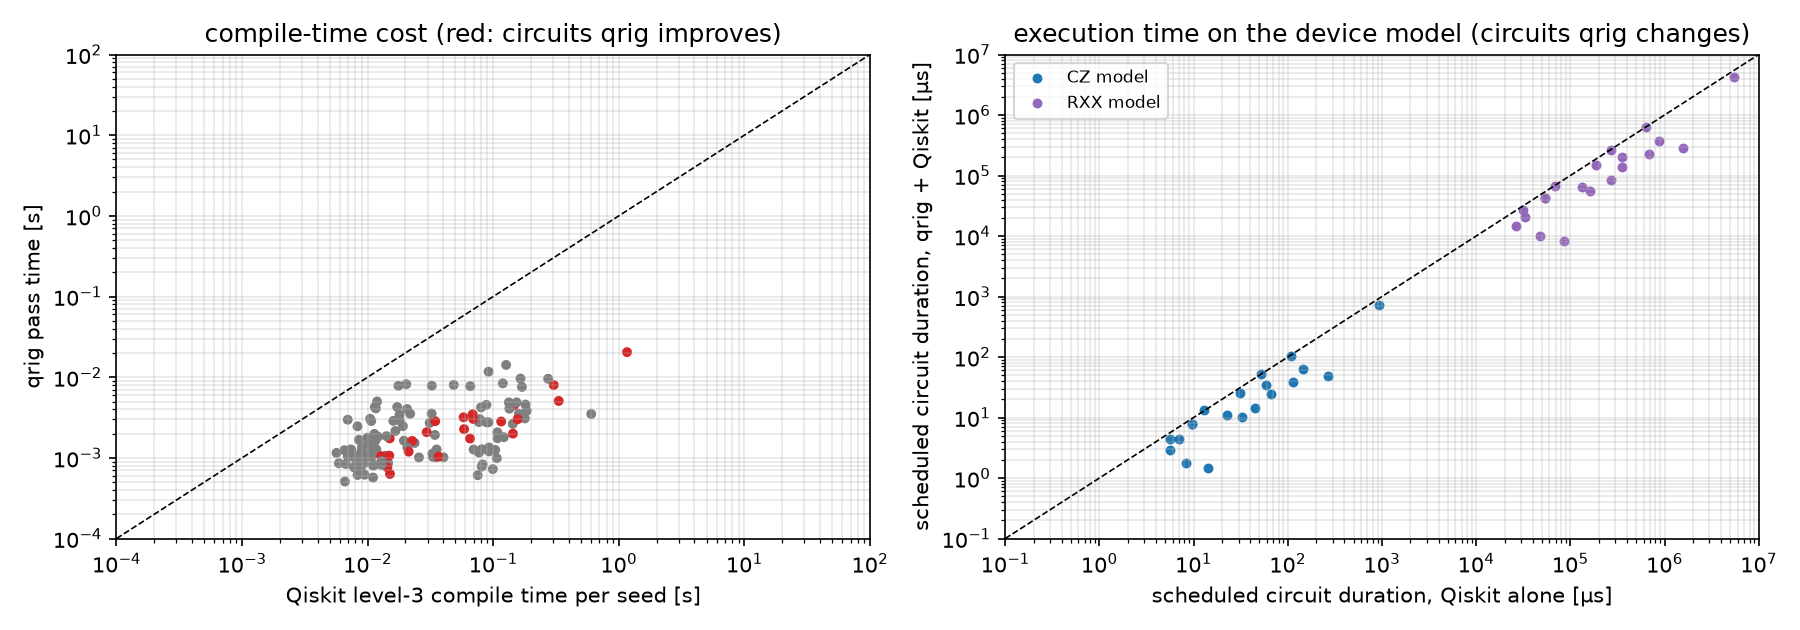
\includegraphics[keepaspectratio,alt={Left: qrig pass time against Qiskit's compile time. Right: scheduled execution time of the compiled circuits on the two device models.}]{figures/fig5_time.png}}
\caption{Left: qrig pass time against Qiskit's compile time. Right:
scheduled execution time of the compiled circuits on the two device
models.}
\end{figure}

\begin{itemize}
\tightlist
\item
  \textbf{Compile-time cost.} qrig pass: median 1.7 ms, maximum 0.02 s
  per circuit. Qiskit level 3 (one seed, CZ model): median 21.5 ms,
  maximum 1.16 s. Median ratio qrig/Qiskit 0.07.
\item
  \textbf{Execution time on the device.} Removing gates also shortens
  the scheduled circuit, so each shot runs faster and (Section 5) fewer
  shots are needed:
\end{itemize}

{\def\LTcaptype{none} % do not increment counter
\begin{longtable}[]{@{}
  >{\raggedright\arraybackslash}p{(\linewidth - 4\tabcolsep) * \real{0.3333}}
  >{\raggedright\arraybackslash}p{(\linewidth - 4\tabcolsep) * \real{0.3333}}
  >{\raggedright\arraybackslash}p{(\linewidth - 4\tabcolsep) * \real{0.3333}}@{}}
\toprule\noalign{}
\begin{minipage}[b]{\linewidth}\raggedright
circuit
\end{minipage} & \begin{minipage}[b]{\linewidth}\raggedright
duration, CZ model
\end{minipage} & \begin{minipage}[b]{\linewidth}\raggedright
duration, RXX model
\end{minipage} \\
\midrule\noalign{}
\endhead
\bottomrule\noalign{}
\endlastfoot
grover 4 & 5.7 \ensuremath{\rightarrow} 4.5 \ensuremath{\mu}s (-21 \%) & 31.4 \ensuremath{\rightarrow} 27.4 ms (-13 \%) \\
grover 7 & 107.8 \ensuremath{\rightarrow} 105.1 \ensuremath{\mu}s (-2 \%) & 631.4 \ensuremath{\rightarrow} 623.0 ms (-1 \%) \\
grover 10 & 925.0 \ensuremath{\rightarrow} 720.6 \ensuremath{\mu}s (-22 \%) & 5502.0 \ensuremath{\rightarrow} 4267.9 ms (-22 \%) \\
hrs\_cumulative\_multiplier 5 & 12.9 \ensuremath{\rightarrow} 13.6 \ensuremath{\mu}s (+5 \%) & 68.2 \ensuremath{\rightarrow} 67.4 ms
(-1 \%) \\
hrs\_cumulative\_multiplier 9 & 51.8 \ensuremath{\rightarrow} 52.5 \ensuremath{\mu}s (+1 \%) & 269.0 \ensuremath{\rightarrow} 264.2
ms (-2 \%) \\
multiplier 8 & 9.6 \ensuremath{\rightarrow} 7.8 \ensuremath{\mu}s (-19 \%) & 54.4 \ensuremath{\rightarrow} 43.1 ms (-21 \%) \\
rg\_qft\_multiplier 8 & 9.6 \ensuremath{\rightarrow} 7.8 \ensuremath{\mu}s (-19 \%) & 54.4 \ensuremath{\rightarrow} 43.1 ms (-21
\%) \\
qrom 2x3 & 5.6 \ensuremath{\rightarrow} 2.9 \ensuremath{\mu}s (-48 \%) & 26.6 \ensuremath{\rightarrow} 14.6 ms (-45 \%) \\
qrom 3x3 & 22.7 \ensuremath{\rightarrow} 11.2 \ensuremath{\mu}s (-51 \%) & 134.2 \ensuremath{\rightarrow} 65.4 ms (-51 \%) \\
qrom 3x5 & 45.1 \ensuremath{\rightarrow} 14.4 \ensuremath{\mu}s (-68 \%) & 268.1 \ensuremath{\rightarrow} 84.0 ms (-69 \%) \\
qrom 4x4 & 113.4 \ensuremath{\rightarrow} 38.9 \ensuremath{\mu}s (-66 \%) & 676.0 \ensuremath{\rightarrow} 230.9 ms (-66 \%) \\
lcu\_select 2x3 & 7.1 \ensuremath{\rightarrow} 4.3 \ensuremath{\mu}s (-39 \%) & 32.9 \ensuremath{\rightarrow} 20.9 ms (-36 \%) \\
lcu\_select 3x3 & 31.2 \ensuremath{\rightarrow} 25.6 \ensuremath{\mu}s (-18 \%) & 185.7 \ensuremath{\rightarrow} 151.7 ms (-18 \%) \\
lcu\_select 3x5 & 58.8 \ensuremath{\rightarrow} 34.7 \ensuremath{\mu}s (-41 \%) & 350.5 \ensuremath{\rightarrow} 206.1 ms (-41 \%) \\
membership\_oracle 4 & 32.6 \ensuremath{\rightarrow} 10.4 \ensuremath{\mu}s (-68 \%) & 161.8 \ensuremath{\rightarrow} 55.0 ms (-66
\%) \\
membership\_oracle 6 & 146.4 \ensuremath{\rightarrow} 62.7 \ensuremath{\mu}s (-57 \%) & 881.6 \ensuremath{\rightarrow} 373.7 ms (-58
\%) \\
multiplexer (3 controls) & 14.3 \ensuremath{\rightarrow} 1.5 \ensuremath{\mu}s (-90 \%) & 85.5 \ensuremath{\rightarrow} 8.2 ms (-90
\%) \\
multiplexer (4 controls) & 65.8 \ensuremath{\rightarrow} 24.4 \ensuremath{\mu}s (-63 \%) & 351.2 \ensuremath{\rightarrow} 137.3 ms
(-61 \%) \\
multiplexer (5 controls) & 265.4 \ensuremath{\rightarrow} 49.1 \ensuremath{\mu}s (-81 \%) & 1582.1 \ensuremath{\rightarrow} 283.7 ms
(-82 \%) \\
C3(T) x4 & 8.4 \ensuremath{\rightarrow} 1.8 \ensuremath{\mu}s (-79 \%) & 47.9 \ensuremath{\rightarrow} 10.2 ms (-79 \%) \\
compute/uncompute U;U\^{}-1 & 36.5 \ensuremath{\rightarrow} 0.0 \ensuremath{\mu}s (-100 \%) & 195.8 \ensuremath{\rightarrow} 0.0 ms
(-100 \%) \\
C3(H);C3(V);C3(V\^{}-1);C3(H) & 7.4 \ensuremath{\rightarrow} 0.0 \ensuremath{\mu}s (-100 \%) & 41.0 \ensuremath{\rightarrow} 0.0 ms
(-100 \%) \\
\end{longtable}
}

Time-to-solution for a fixed precision scales roughly like duration \ensuremath{\times}
1/F\textsuperscript{2} (ignoring fixed per-shot overheads such as reset and readout); both
factors fall with qrig on the circuits above.

\section{7. Fault-tolerant cost
(T-count)}\label{fault-tolerant-cost-t-count}

Both pipelines compiled with Qiskit level 3 to \{cx, h, s, sdg, t, tdg,
x, z, rz\}; \texttt{rz} angles that are odd multiples of \ensuremath{\pi}/4 count as T,
other non-Clifford angles as \emph{arbitrary rotations} (each costs tens
of T gates after synthesis).

{\def\LTcaptype{none} % do not increment counter
\begin{longtable}[]{@{}llll@{}}
\toprule\noalign{}
circuit & T-count & arbitrary rotations & CX \\
\midrule\noalign{}
\endhead
\bottomrule\noalign{}
\endlastfoot
grover 4 & 46 \ensuremath{\rightarrow} 13 & 14 \ensuremath{\rightarrow} 35 & 52 \ensuremath{\rightarrow} 38 \\
grover 7 & 630 \ensuremath{\rightarrow} 558 & 618 \ensuremath{\rightarrow} 570 & 1092 \ensuremath{\rightarrow} 996 \\
grover 10 & 7650 \ensuremath{\rightarrow} 4301 & 2431 \ensuremath{\rightarrow} 3825 & 8874 \ensuremath{\rightarrow} 6970 \\
hrs\_cumulative\_multiplier 5 & 100 \ensuremath{\rightarrow} 100 & 44 \ensuremath{\rightarrow} 43 & 124 \ensuremath{\rightarrow} 124 \\
hrs\_cumulative\_multiplier 9 & 392 \ensuremath{\rightarrow} 392 & 172 \ensuremath{\rightarrow} 175 & 488 \ensuremath{\rightarrow} 486 \\
multiplier 8 & 37 \ensuremath{\rightarrow} 37 & 64 \ensuremath{\rightarrow} 64 & 120 \ensuremath{\rightarrow} 96 \\
rg\_qft\_multiplier 8 & 37 \ensuremath{\rightarrow} 37 & 64 \ensuremath{\rightarrow} 64 & 120 \ensuremath{\rightarrow} 96 \\
qrom 2x3 & 50 \ensuremath{\rightarrow} 26 & 0 \ensuremath{\rightarrow} 0 & 48 \ensuremath{\rightarrow} 26 \\
qrom 3x3 & 3 \ensuremath{\rightarrow} 27 & 187 \ensuremath{\rightarrow} 71 & 182 \ensuremath{\rightarrow} 92 \\
qrom 3x5 & 2 \ensuremath{\rightarrow} 38 & 368 \ensuremath{\rightarrow} 89 & 364 \ensuremath{\rightarrow} 122 \\
qrom 4x4 & 1008 \ensuremath{\rightarrow} 180 & 0 \ensuremath{\rightarrow} 164 & 936 \ensuremath{\rightarrow} 322 \\
lcu\_select 2x3 & 62 \ensuremath{\rightarrow} 40 & 0 \ensuremath{\rightarrow} 0 & 60 \ensuremath{\rightarrow} 38 \\
lcu\_select 3x3 & 2 \ensuremath{\rightarrow} 13 & 258 \ensuremath{\rightarrow} 202 & 252 \ensuremath{\rightarrow} 208 \\
lcu\_select 3x5 & 0 \ensuremath{\rightarrow} 49 & 482 \ensuremath{\rightarrow} 270 & 476 \ensuremath{\rightarrow} 289 \\
membership\_oracle 4 & 176 \ensuremath{\rightarrow} 51 & 165 \ensuremath{\rightarrow} 55 & 288 \ensuremath{\rightarrow} 92 \\
membership\_oracle 6 & 456 \ensuremath{\rightarrow} 290 & 1136 \ensuremath{\rightarrow} 379 & 1488 \ensuremath{\rightarrow} 606 \\
multiplexer (3 controls) & 26 \ensuremath{\rightarrow} 9 & 106 \ensuremath{\rightarrow} 7 & 124 \ensuremath{\rightarrow} 13 \\
multiplexer (4 controls) & 438 \ensuremath{\rightarrow} 153 & 286 \ensuremath{\rightarrow} 117 & 624 \ensuremath{\rightarrow} 234 \\
multiplexer (5 controls) & 1606 \ensuremath{\rightarrow} 369 & 1347 \ensuremath{\rightarrow} 159 & 2688 \ensuremath{\rightarrow} 454 \\
C3(T) x4 & 48 \ensuremath{\rightarrow} 4 & 41 \ensuremath{\rightarrow} 17 & 80 \ensuremath{\rightarrow} 14 \\
compute/uncompute U;U\^{}-1 & 202 \ensuremath{\rightarrow} 0 & 193 \ensuremath{\rightarrow} 0 & 349 \ensuremath{\rightarrow} 0 \\
C3(H);C3(V);C3(V\^{}-1);C3(H) & 14 \ensuremath{\rightarrow} 0 & 60 \ensuremath{\rightarrow} 0 & 66 \ensuremath{\rightarrow} 0 \\
\end{longtable}
}

qrig lowers the T-count on 14 of the 22 circuits it changes. On 4
circuits (grover 4, grover 10, hrs\_cumulative\_multiplier 9, qrom 4x4)
it \emph{increases} the number of arbitrary rotations: Qiskit
synthesises the multi-controlled gates that qrig emits (e.g.~C\textsuperscript{3}Z instead
of a multi-controlled phase of \ensuremath{\pi}) without ancillas, using \ensuremath{\pi}/8-type
rotations. This is a property of Qiskit's ancilla-free synthesis, not of
the rewrite; T-count is therefore a mixed metric for qrig today and an
open improvement (emit the multi-controlled gates in the form Qiskit
synthesises best).

\section{8. Robustness}\label{robustness}

\subsection{8.1 Across compiler randomness (transpiler
seeds)}\label{across-compiler-randomness-transpiler-seeds}

{\def\LTcaptype{none} % do not increment counter
\begin{longtable}[]{@{}
  >{\raggedright\arraybackslash}p{(\linewidth - 8\tabcolsep) * \real{0.2000}}
  >{\raggedright\arraybackslash}p{(\linewidth - 8\tabcolsep) * \real{0.2000}}
  >{\raggedright\arraybackslash}p{(\linewidth - 8\tabcolsep) * \real{0.2000}}
  >{\raggedright\arraybackslash}p{(\linewidth - 8\tabcolsep) * \real{0.2000}}
  >{\raggedright\arraybackslash}p{(\linewidth - 8\tabcolsep) * \real{0.2000}}@{}}
\toprule\noalign{}
\begin{minipage}[b]{\linewidth}\raggedright
circuit
\end{minipage} & \begin{minipage}[b]{\linewidth}\raggedright
2q min/median/max, CX
\end{minipage} & \begin{minipage}[b]{\linewidth}\raggedright
CZ
\end{minipage} & \begin{minipage}[b]{\linewidth}\raggedright
RXX
\end{minipage} & \begin{minipage}[b]{\linewidth}\raggedright
seeds no worse (CZ)
\end{minipage} \\
\midrule\noalign{}
\endhead
\bottomrule\noalign{}
\endlastfoot
grover 4 & 52/52/52 \ensuremath{\rightarrow} 38/38/38 & 52/52/52 \ensuremath{\rightarrow} 38/38/38 & 44/44/44 \ensuremath{\rightarrow}
36/36/36 & 100 \% \\
grover 7 & 1092/1092/1092 \ensuremath{\rightarrow} 996/996/996 & 1092/1092/1092 \ensuremath{\rightarrow} 996/996/996 &
990/990/990 \ensuremath{\rightarrow} 918/918/918 & 100 \% \\
grover 10 & 8874/8874/8874 \ensuremath{\rightarrow} 6970/6970/6970 & 8874/8874/8874 \ensuremath{\rightarrow}
6970/6970/6970 & 8211/8211/8211 \ensuremath{\rightarrow} 6477/6477/6477 & 100 \% \\
hrs\_cumulative\_multiplier 5 & 122/122/122 \ensuremath{\rightarrow} 122/122/122 & 122/122/122
\ensuremath{\rightarrow} 128/128/128 & 91/91/91 \ensuremath{\rightarrow} 90/90/90 & 0 \% \\
hrs\_cumulative\_multiplier 9 & 484/484/484 \ensuremath{\rightarrow} 482/482/482 & 484/484/484
\ensuremath{\rightarrow} 494/494/494 & 358/358/358 \ensuremath{\rightarrow} 352/352/352 & 0 \% \\
multiplier 8 & 115/115/115 \ensuremath{\rightarrow} 96/96/96 & 115/115/115 \ensuremath{\rightarrow} 96/96/96 &
91/91/91 \ensuremath{\rightarrow} 72/72/72 & 100 \% \\
rg\_qft\_multiplier 8 & 115/115/115 \ensuremath{\rightarrow} 96/96/96 & 115/115/115 \ensuremath{\rightarrow} 96/96/96
& 91/91/91 \ensuremath{\rightarrow} 72/72/72 & 100 \% \\
qrom 2x3 & 48/48/48 \ensuremath{\rightarrow} 26/26/26 & 48/48/48 \ensuremath{\rightarrow} 26/26/26 & 40/40/40 \ensuremath{\rightarrow}
21/21/21 & 100 \% \\
qrom 3x3 & 182/182/182 \ensuremath{\rightarrow} 92/92/92 & 182/182/182 \ensuremath{\rightarrow} 92/92/92 & 169/169/169
\ensuremath{\rightarrow} 85/85/85 & 100 \% \\
qrom 3x5 & 364/364/364 \ensuremath{\rightarrow} 122/122/122 & 364/364/364 \ensuremath{\rightarrow} 122/122/122 &
338/338/338 \ensuremath{\rightarrow} 110/110/110 & 100 \% \\
qrom 4x4 & 936/936/936 \ensuremath{\rightarrow} 322/322/322 & 936/936/936 \ensuremath{\rightarrow} 322/322/322 &
864/864/864 \ensuremath{\rightarrow} 297/297/297 & 100 \% \\
lcu\_select 2x3 & 60/60/60 \ensuremath{\rightarrow} 38/38/38 & 60/60/60 \ensuremath{\rightarrow} 38/38/38 & 50/50/50 \ensuremath{\rightarrow}
32/32/32 & 100 \% \\
lcu\_select 3x3 & 252/252/252 \ensuremath{\rightarrow} 208/208/208 & 252/252/252 \ensuremath{\rightarrow} 208/208/208
& 234/234/234 \ensuremath{\rightarrow} 192/192/192 & 100 \% \\
lcu\_select 3x5 & 476/476/476 \ensuremath{\rightarrow} 289/289/289 & 476/476/476 \ensuremath{\rightarrow} 289/289/289
& 442/442/442 \ensuremath{\rightarrow} 265/265/265 & 100 \% \\
membership\_oracle 4 & 288/288/288 \ensuremath{\rightarrow} 92/92/92 & 288/288/288 \ensuremath{\rightarrow} 92/92/92 &
216/216/216 \ensuremath{\rightarrow} 72/72/72 & 100 \% \\
membership\_oracle 6 & 1488/1488/1488 \ensuremath{\rightarrow} 606/606/606 & 1488/1488/1488 \ensuremath{\rightarrow}
606/606/606 & 1356/1356/1356 \ensuremath{\rightarrow} 556/556/556 & 100 \% \\
multiplexer (3 controls) & 122/122/122 \ensuremath{\rightarrow} 12/12/12 & 122/122/122 \ensuremath{\rightarrow}
12/12/12 & 111/111/111 \ensuremath{\rightarrow} 10/10/10 & 100 \% \\
multiplexer (4 controls) & 624/624/624 \ensuremath{\rightarrow} 232/232/232 & 624/624/624 \ensuremath{\rightarrow}
232/232/232 & 492/492/492 \ensuremath{\rightarrow} 192/192/192 & 100 \% \\
multiplexer (5 controls) & 2626/2626/2626 \ensuremath{\rightarrow} 452/452/452 & 2626/2626/2626
\ensuremath{\rightarrow} 452/452/452 & 2305/2305/2305 \ensuremath{\rightarrow} 399/399/399 & 100 \% \\
C3(T) x4 & 80/80/80 \ensuremath{\rightarrow} 14/14/14 & 80/80/80 \ensuremath{\rightarrow} 14/14/14 & 68/68/68 \ensuremath{\rightarrow}
13/13/13 & 100 \% \\
compute/uncompute U;U\^{}-1 & 343/343/343 \ensuremath{\rightarrow} 0/0/0 & 343/343/343 \ensuremath{\rightarrow} 0/0/0
& 272/272/272 \ensuremath{\rightarrow} 0/0/0 & 100 \% \\
C3(H);C3(V);C3(V\^{}-1);C3(H) & 64/64/64 \ensuremath{\rightarrow} 0/0/0 & 64/64/64 \ensuremath{\rightarrow} 0/0/0 &
54/54/54 \ensuremath{\rightarrow} 0/0/0 & 100 \% \\
\end{longtable}
}

Over all 3900 (circuit, target, seed) compilations, qrig + Qiskit used
no more two-qubit gates than Qiskit alone with the same seed in 3880
(99.5 \%).

Note: with all-to-all connectivity there is no layout or routing step,
which is where Qiskit's randomness mostly acts; the two-qubit count
varies across seeds in only 0 of the 780 (circuit, target, pipeline)
combinations. Seed robustness is therefore close to automatic here; it
becomes a real test on a restricted topology (Section 10).

\subsection{8.2 Across noise strength}\label{across-noise-strength}

Circuits whose CZ-model two-qubit count qrig changes and that have at
most 8 qubits (20 circuits) were re-simulated on the CZ model with every
gate error multiplied, and T1/T2 divided, by a common scale factor (the
compiled circuits are the same; only the noise changes).

\begin{figure}
\centering
\pandocbounded{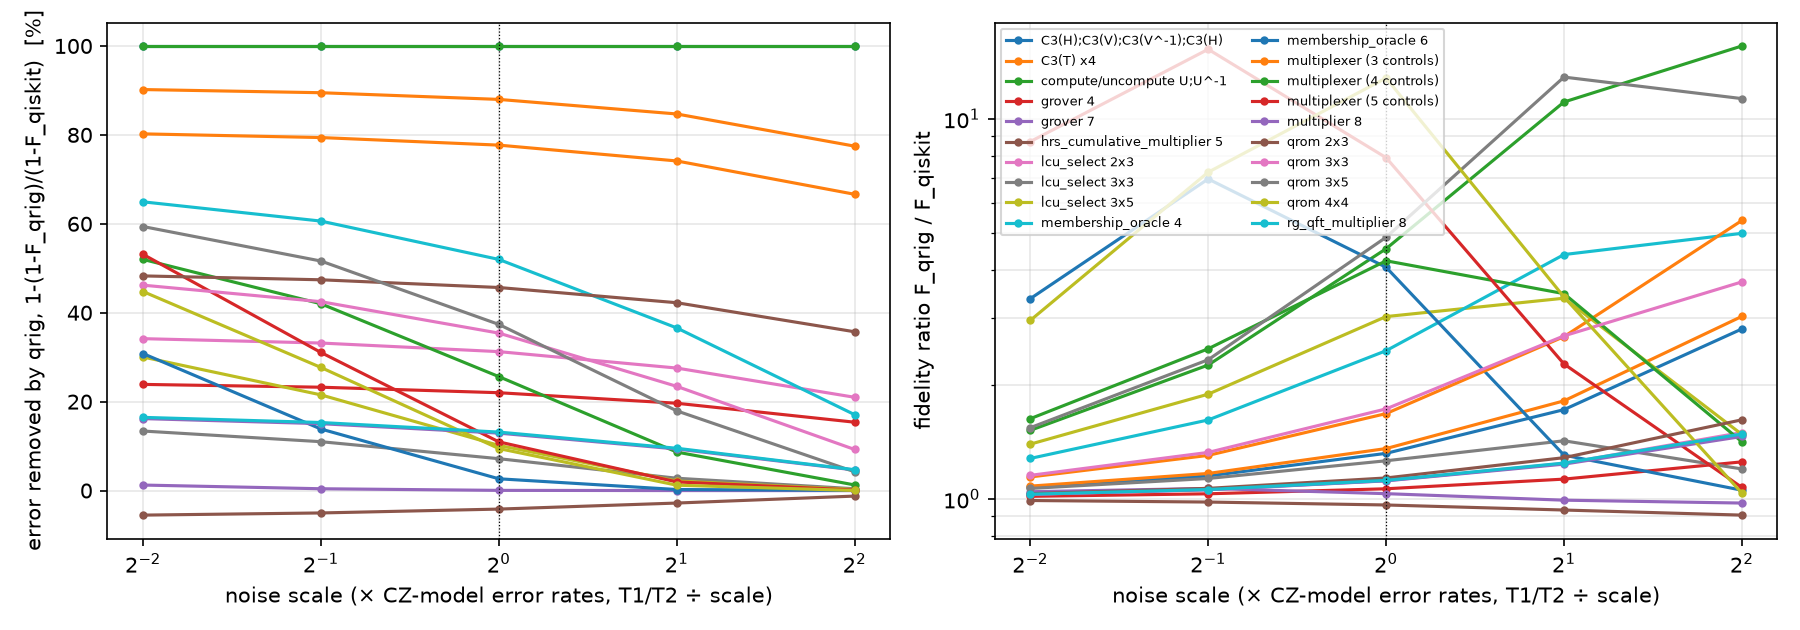
\includegraphics[keepaspectratio,alt={Error removed (left) and fidelity ratio (right) as the noise strength changes.}]{figures/fig3_noise_scale.png}}
\caption{Error removed (left) and fidelity ratio (right) as the noise
strength changes.}
\end{figure}

{\def\LTcaptype{none} % do not increment counter
\begin{longtable}[]{@{}
  >{\raggedright\arraybackslash}p{(\linewidth - 10\tabcolsep) * \real{0.1667}}
  >{\raggedright\arraybackslash}p{(\linewidth - 10\tabcolsep) * \real{0.1667}}
  >{\raggedright\arraybackslash}p{(\linewidth - 10\tabcolsep) * \real{0.1667}}
  >{\raggedright\arraybackslash}p{(\linewidth - 10\tabcolsep) * \real{0.1667}}
  >{\raggedright\arraybackslash}p{(\linewidth - 10\tabcolsep) * \real{0.1667}}
  >{\raggedright\arraybackslash}p{(\linewidth - 10\tabcolsep) * \real{0.1667}}@{}}
\toprule\noalign{}
\begin{minipage}[b]{\linewidth}\raggedright
circuit
\end{minipage} & \begin{minipage}[b]{\linewidth}\raggedright
scale 0.25
\end{minipage} & \begin{minipage}[b]{\linewidth}\raggedright
scale 0.5
\end{minipage} & \begin{minipage}[b]{\linewidth}\raggedright
scale 1
\end{minipage} & \begin{minipage}[b]{\linewidth}\raggedright
scale 2
\end{minipage} & \begin{minipage}[b]{\linewidth}\raggedright
scale 4
\end{minipage} \\
\midrule\noalign{}
\endhead
\bottomrule\noalign{}
\endlastfoot
C3(H);C3(V);C3(V\^{}-1);C3(H) & +100 \% (\ensuremath{\times}1.07) & +100 \% (\ensuremath{\times}1.15) & +100
\% (\ensuremath{\times}1.32) & +100 \% (\ensuremath{\times}1.72) & +100 \% (\ensuremath{\times}2.80) \\
C3(T) x4 & +80 \% (\ensuremath{\times}1.08) & +79 \% (\ensuremath{\times}1.17) & +78 \% (\ensuremath{\times}1.36) & +74 \%
(\ensuremath{\times}1.81) & +67 \% (\ensuremath{\times}3.02) \\
compute/uncompute U;U\^{}-1 & +100 \% (\ensuremath{\times}1.52) & +100 \% (\ensuremath{\times}2.25) & +100
\% (\ensuremath{\times}4.55) & +100 \% (\ensuremath{\times}11.08) & +100 \% (\ensuremath{\times}15.56) \\
grover 4 & +24 \% (\ensuremath{\times}1.02) & +23 \% (\ensuremath{\times}1.03) & +22 \% (\ensuremath{\times}1.06) & +20 \%
(\ensuremath{\times}1.13) & +15 \% (\ensuremath{\times}1.25) \\
grover 7 & +1 \% (\ensuremath{\times}1.04) & +0 \% (\ensuremath{\times}1.07) & +0 \% (\ensuremath{\times}1.03) & -0 \% (\ensuremath{\times}0.99)
& -0 \% (\ensuremath{\times}0.98) \\
hrs\_cumulative\_multiplier 5 & -6 \% (\ensuremath{\times}0.99) & -5 \% (\ensuremath{\times}0.98) & -4 \%
(\ensuremath{\times}0.96) & -3 \% (\ensuremath{\times}0.93) & -1 \% (\ensuremath{\times}0.91) \\
lcu\_select 2x3 & +34 \% (\ensuremath{\times}1.03) & +33 \% (\ensuremath{\times}1.06) & +31 \% (\ensuremath{\times}1.12) & +28
\% (\ensuremath{\times}1.24) & +21 \% (\ensuremath{\times}1.50) \\
lcu\_select 3x3 & +13 \% (\ensuremath{\times}1.07) & +11 \% (\ensuremath{\times}1.13) & +7 \% (\ensuremath{\times}1.26) & +3
\% (\ensuremath{\times}1.42) & +0 \% (\ensuremath{\times}1.20) \\
lcu\_select 3x5 & +30 \% (\ensuremath{\times}1.39) & +22 \% (\ensuremath{\times}1.89) & +10 \% (\ensuremath{\times}3.02) & +2
\% (\ensuremath{\times}3.37) & +0 \% (\ensuremath{\times}1.48) \\
membership\_oracle 4 & +65 \% (\ensuremath{\times}1.28) & +61 \% (\ensuremath{\times}1.61) & +52 \% (\ensuremath{\times}2.46)
& +37 \% (\ensuremath{\times}4.40) & +17 \% (\ensuremath{\times}5.00) \\
membership\_oracle 6 & +31 \% (\ensuremath{\times}3.36) & +14 \% (\ensuremath{\times}6.95) & +3 \% (\ensuremath{\times}4.07) &
+0 \% (\ensuremath{\times}1.30) & +0 \% (\ensuremath{\times}1.05) \\
multiplexer (3 controls) & +90 \% (\ensuremath{\times}1.14) & +89 \% (\ensuremath{\times}1.30) & +88 \%
(\ensuremath{\times}1.68) & +85 \% (\ensuremath{\times}2.67) & +77 \% (\ensuremath{\times}5.41) \\
multiplexer (4 controls) & +52 \% (\ensuremath{\times}1.63) & +42 \% (\ensuremath{\times}2.48) & +26 \%
(\ensuremath{\times}4.23) & +9 \% (\ensuremath{\times}3.47) & +1 \% (\ensuremath{\times}1.41) \\
multiplexer (5 controls) & +53 \% (\ensuremath{\times}8.72) & +31 \% (\ensuremath{\times}15.25) & +11 \%
(\ensuremath{\times}7.91) & +2 \% (\ensuremath{\times}2.27) & +0 \% (\ensuremath{\times}1.07) \\
multiplier 8 & +16 \% (\ensuremath{\times}1.03) & +15 \% (\ensuremath{\times}1.06) & +13 \% (\ensuremath{\times}1.12) & +9 \%
(\ensuremath{\times}1.23) & +5 \% (\ensuremath{\times}1.46) \\
qrom 2x3 & +48 \% (\ensuremath{\times}1.03) & +47 \% (\ensuremath{\times}1.07) & +46 \% (\ensuremath{\times}1.14) & +42 \%
(\ensuremath{\times}1.28) & +36 \% (\ensuremath{\times}1.62) \\
qrom 3x3 & +46 \% (\ensuremath{\times}1.15) & +42 \% (\ensuremath{\times}1.33) & +35 \% (\ensuremath{\times}1.73) & +23 \%
(\ensuremath{\times}2.69) & +9 \% (\ensuremath{\times}3.73) \\
qrom 3x5 & +59 \% (\ensuremath{\times}1.54) & +52 \% (\ensuremath{\times}2.32) & +37 \% (\ensuremath{\times}4.88) & +18 \%
(\ensuremath{\times}12.89) & +4 \% (\ensuremath{\times}11.31) \\
qrom 4x4 & +45 \% (\ensuremath{\times}2.95) & +28 \% (\ensuremath{\times}7.24) & +9 \% (\ensuremath{\times}12.81) & +1 \%
(\ensuremath{\times}3.40) & +0 \% (\ensuremath{\times}1.04) \\
rg\_qft\_multiplier 8 & +16 \% (\ensuremath{\times}1.03) & +15 \% (\ensuremath{\times}1.06) & +13 \% (\ensuremath{\times}1.12)
& +10 \% (\ensuremath{\times}1.24) & +5 \% (\ensuremath{\times}1.48) \\
\end{longtable}
}

\subsection{8.3 Across noise type}\label{across-noise-type}

\begin{figure}
\centering
\pandocbounded{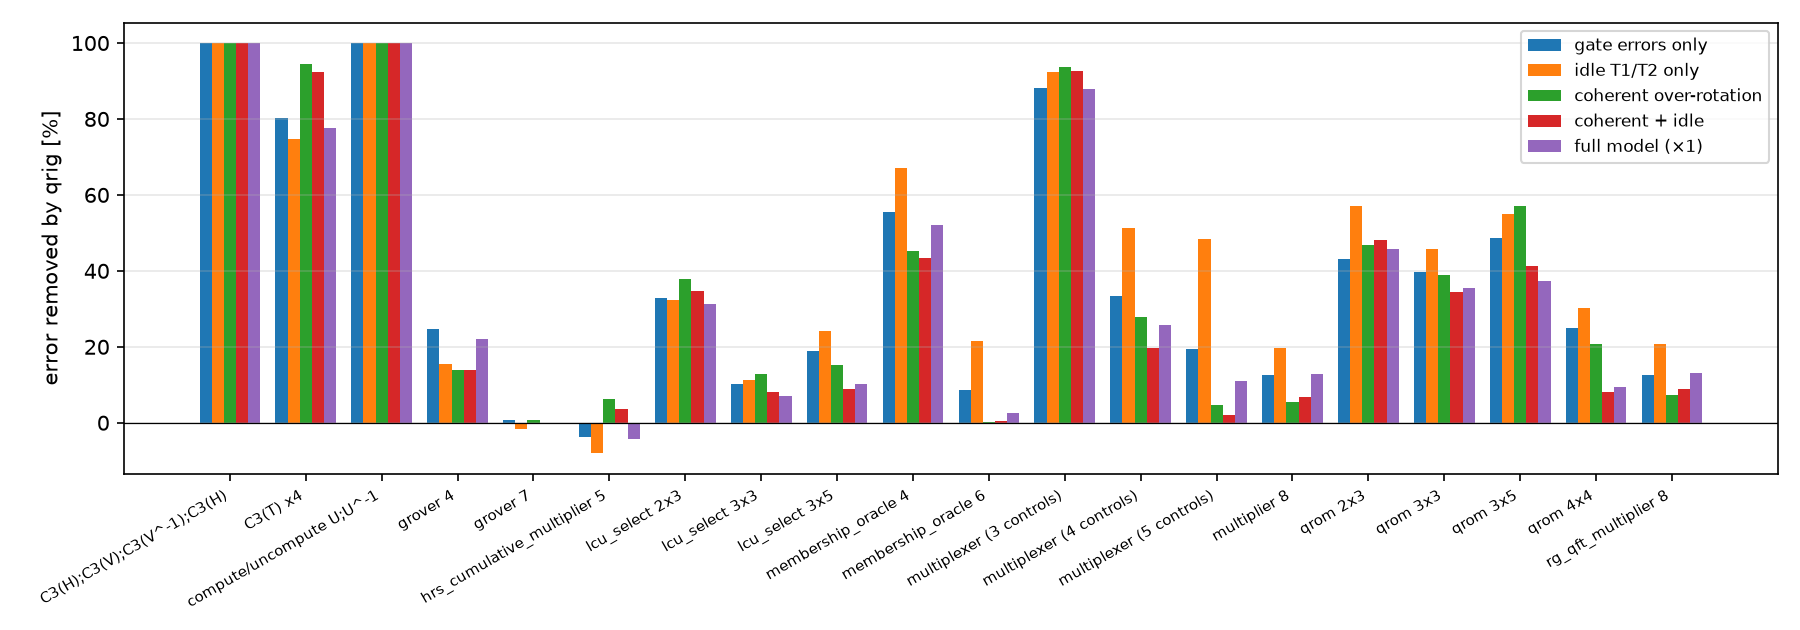
\includegraphics[keepaspectratio,alt={Error removed under different kinds of noise (same compiled circuits).}]{figures/fig4_noise_type.png}}
\caption{Error removed under different kinds of noise (same compiled
circuits).}
\end{figure}

{\def\LTcaptype{none} % do not increment counter
\begin{longtable}[]{@{}
  >{\raggedright\arraybackslash}p{(\linewidth - 8\tabcolsep) * \real{0.2000}}
  >{\raggedright\arraybackslash}p{(\linewidth - 8\tabcolsep) * \real{0.2000}}
  >{\raggedright\arraybackslash}p{(\linewidth - 8\tabcolsep) * \real{0.2000}}
  >{\raggedright\arraybackslash}p{(\linewidth - 8\tabcolsep) * \real{0.2000}}
  >{\raggedright\arraybackslash}p{(\linewidth - 8\tabcolsep) * \real{0.2000}}@{}}
\toprule\noalign{}
\begin{minipage}[b]{\linewidth}\raggedright
circuit (F: Qiskit \ensuremath{\rightarrow} qrig)
\end{minipage} & \begin{minipage}[b]{\linewidth}\raggedright
gate errors only
\end{minipage} & \begin{minipage}[b]{\linewidth}\raggedright
idle T1/T2 only
\end{minipage} & \begin{minipage}[b]{\linewidth}\raggedright
coherent
\end{minipage} & \begin{minipage}[b]{\linewidth}\raggedright
coherent + idle
\end{minipage} \\
\midrule\noalign{}
\endhead
\bottomrule\noalign{}
\endlastfoot
C3(H);C3(V);C3(V\^{}-1);C3(H) & 0.795 \ensuremath{\rightarrow} 1.000 & 0.952 \ensuremath{\rightarrow} 1.000 & 0.629 \ensuremath{\rightarrow}
1.000 & 0.601 \ensuremath{\rightarrow} 1.000 \\
C3(T) x4 & 0.745 \ensuremath{\rightarrow} 0.949 & 0.918 \ensuremath{\rightarrow} 0.979 & 0.145 \ensuremath{\rightarrow} 0.953 & 0.139 \ensuremath{\rightarrow}
0.933 \\
compute/uncompute U;U\^{}-1 & 0.284 \ensuremath{\rightarrow} 1.000 & 0.721 \ensuremath{\rightarrow} 1.000 & 0.293 \ensuremath{\rightarrow}
1.000 & 0.227 \ensuremath{\rightarrow} 1.000 \\
grover 4 & 0.817 \ensuremath{\rightarrow} 0.862 & 0.949 \ensuremath{\rightarrow} 0.957 & 0.842 \ensuremath{\rightarrow} 0.864 & 0.799 \ensuremath{\rightarrow}
0.827 \\
grover 7 & 0.028 \ensuremath{\rightarrow} 0.034 & 0.141 \ensuremath{\rightarrow} 0.126 & 1.1e-03 \ensuremath{\rightarrow} 9.0e-03 & 7.3e-03 \ensuremath{\rightarrow}
7.9e-03 \\
hrs\_cumulative\_multiplier 5 & 0.627 \ensuremath{\rightarrow} 0.612 & 0.851 \ensuremath{\rightarrow} 0.839 & 0.276 \ensuremath{\rightarrow}
0.322 & 0.242 \ensuremath{\rightarrow} 0.270 \\
lcu\_select 2x3 & 0.794 \ensuremath{\rightarrow} 0.862 & 0.915 \ensuremath{\rightarrow} 0.943 & 0.822 \ensuremath{\rightarrow} 0.889 & 0.754
\ensuremath{\rightarrow} 0.839 \\
lcu\_select 3x3 & 0.369 \ensuremath{\rightarrow} 0.434 & 0.561 \ensuremath{\rightarrow} 0.611 & 0.269 \ensuremath{\rightarrow} 0.362 & 0.167
\ensuremath{\rightarrow} 0.235 \\
lcu\_select 3x5 & 0.160 \ensuremath{\rightarrow} 0.319 & 0.243 \ensuremath{\rightarrow} 0.427 & 0.143 \ensuremath{\rightarrow} 0.273 & 0.041
\ensuremath{\rightarrow} 0.125 \\
membership\_oracle 4 & 0.359 \ensuremath{\rightarrow} 0.715 & 0.697 \ensuremath{\rightarrow} 0.900 & 0.334 \ensuremath{\rightarrow} 0.635 &
0.250 \ensuremath{\rightarrow} 0.575 \\
membership\_oracle 6 & 0.014 \ensuremath{\rightarrow} 0.098 & 0.059 \ensuremath{\rightarrow} 0.261 & 0.015 \ensuremath{\rightarrow} 0.018 &
9.2e-03 \ensuremath{\rightarrow} 0.014 \\
multiplexer (3 controls) & 0.635 \ensuremath{\rightarrow} 0.956 & 0.883 \ensuremath{\rightarrow} 0.991 & 0.501 \ensuremath{\rightarrow} 0.969
& 0.450 \ensuremath{\rightarrow} 0.960 \\
multiplexer (4 controls) & 0.119 \ensuremath{\rightarrow} 0.413 & 0.452 \ensuremath{\rightarrow} 0.732 & 9.9e-03 \ensuremath{\rightarrow}
0.285 & 0.032 \ensuremath{\rightarrow} 0.221 \\
multiplexer (5 controls) & 0.017 \ensuremath{\rightarrow} 0.208 & 0.065 \ensuremath{\rightarrow} 0.518 & 2.1e-03 \ensuremath{\rightarrow}
0.048 & 0.020 \ensuremath{\rightarrow} 0.040 \\
multiplier 8 & 0.647 \ensuremath{\rightarrow} 0.691 & 0.811 \ensuremath{\rightarrow} 0.848 & 0.503 \ensuremath{\rightarrow} 0.530 & 0.409 \ensuremath{\rightarrow}
0.450 \\
qrom 2x3 & 0.829 \ensuremath{\rightarrow} 0.903 & 0.929 \ensuremath{\rightarrow} 0.969 & 0.835 \ensuremath{\rightarrow} 0.912 & 0.777 \ensuremath{\rightarrow}
0.884 \\
qrom 3x3 & 0.488 \ensuremath{\rightarrow} 0.692 & 0.658 \ensuremath{\rightarrow} 0.814 & 0.502 \ensuremath{\rightarrow} 0.696 & 0.344 \ensuremath{\rightarrow}
0.570 \\
qrom 3x5 & 0.252 \ensuremath{\rightarrow} 0.615 & 0.316 \ensuremath{\rightarrow} 0.691 & 0.182 \ensuremath{\rightarrow} 0.649 & 0.069 \ensuremath{\rightarrow}
0.453 \\
qrom 4x4 & 0.031 \ensuremath{\rightarrow} 0.274 & 0.063 \ensuremath{\rightarrow} 0.347 & 8.6e-03 \ensuremath{\rightarrow} 0.214 & 6.8e-03 \ensuremath{\rightarrow}
0.086 \\
rg\_qft\_multiplier 8 & 0.646 \ensuremath{\rightarrow} 0.690 & 0.808 \ensuremath{\rightarrow} 0.848 & 0.533 \ensuremath{\rightarrow} 0.568 &
0.433 \ensuremath{\rightarrow} 0.483 \\
\end{longtable}
}

\emph{Coherent}: every two-qubit gate is followed by an unwanted RZZ(0.1
rad) and every \texttt{sx}/\texttt{x} by RX(0.02 rad), no stochastic
noise. Coherent errors can add up or cancel depending on the circuit, so
this is the hardest case for any claim of the form ``fewer gates \ensuremath{\Rightarrow}
higher fidelity''.

Across all 180 (circuit, noise variant) simulations the qrig circuit has
the higher fidelity in 170; the exceptions are grover 7 (scaled 2:
7.3e-03 \ensuremath{\rightarrow} 7.2e-03); grover 7 (scaled 4: 7.0e-03 \ensuremath{\rightarrow} 6.8e-03); grover 7
(idle\_only 1: 0.141 \ensuremath{\rightarrow} 0.126); hrs\_cumulative\_multiplier 5 (scaled
0.25: 0.853 \ensuremath{\rightarrow} 0.845); hrs\_cumulative\_multiplier 5 (scaled 0.5: 0.729 \ensuremath{\rightarrow}
0.716); hrs\_cumulative\_multiplier 5 (scaled 1: 0.537 \ensuremath{\rightarrow} 0.518);
hrs\_cumulative\_multiplier 5 (scaled 2: 0.302 \ensuremath{\rightarrow} 0.282);
hrs\_cumulative\_multiplier 5 (scaled 4: 0.118 \ensuremath{\rightarrow} 0.107);
hrs\_cumulative\_multiplier 5 (gates\_only 1: 0.627 \ensuremath{\rightarrow} 0.612);
hrs\_cumulative\_multiplier 5 (idle\_only 1: 0.851 \ensuremath{\rightarrow} 0.839).

\section{9. qrig in front of other compilers: TKET and
BQSKit}\label{qrig-in-front-of-other-compilers-tket-and-bqskit}

Is the benefit specific to Qiskit? We put qrig in front of two other
optimising compilers --- \textbf{TKET} (pytket 2.18.5,
\texttt{FullPeepholeOptimise}, its strongest generic optimisation) and
\textbf{BQSKit} (1.2.1, \texttt{compile} at optimisation level 2: block
partitioning and numerical resynthesis, \ensuremath{\varepsilon} = 10\textsuperscript{\ensuremath{-}}\textsuperscript{8}) --- and compare
\emph{X alone} with \emph{qrig + X} for each. Target: all-to-all, \{cx,
rz, sx, x\}; noise: the depolarizing model (p2 = 0.3 \%, p1 = 0.03 \%).
BQSKit was run on circuits with at most 8 qubits (numerical synthesis is
slow). Qiskit numbers are those of Sections 4--5. Source:
\texttt{python/benchmarks/compilers\_study.py}.

{\def\LTcaptype{none} % do not increment counter
\begin{longtable}[]{@{}
  >{\raggedright\arraybackslash}p{(\linewidth - 12\tabcolsep) * \real{0.1429}}
  >{\raggedright\arraybackslash}p{(\linewidth - 12\tabcolsep) * \real{0.1429}}
  >{\raggedright\arraybackslash}p{(\linewidth - 12\tabcolsep) * \real{0.1429}}
  >{\raggedright\arraybackslash}p{(\linewidth - 12\tabcolsep) * \real{0.1429}}
  >{\raggedright\arraybackslash}p{(\linewidth - 12\tabcolsep) * \real{0.1429}}
  >{\raggedright\arraybackslash}p{(\linewidth - 12\tabcolsep) * \real{0.1429}}
  >{\raggedright\arraybackslash}p{(\linewidth - 12\tabcolsep) * \real{0.1429}}@{}}
\toprule\noalign{}
\begin{minipage}[b]{\linewidth}\raggedright
compiler X
\end{minipage} & \begin{minipage}[b]{\linewidth}\raggedright
circuits
\end{minipage} & \begin{minipage}[b]{\linewidth}\raggedright
qrig + X fewer 2q
\end{minipage} & \begin{minipage}[b]{\linewidth}\raggedright
equal
\end{minipage} & \begin{minipage}[b]{\linewidth}\raggedright
more
\end{minipage} & \begin{minipage}[b]{\linewidth}\raggedright
total 2q: X \ensuremath{\rightarrow} qrig + X
\end{minipage} & \begin{minipage}[b]{\linewidth}\raggedright
change
\end{minipage} \\
\midrule\noalign{}
\endhead
\bottomrule\noalign{}
\endlastfoot
Qiskit O3 & 130 & 21 & 109 & 0 & 29398 \ensuremath{\rightarrow} 21896 & -25.5 \% \\
TKET & 130 & 17 & 112 & 1 & 31933 \ensuremath{\rightarrow} 26305 & -17.6 \% \\
BQSKit & 93 & 24 & 69 & 0 & 10697 \ensuremath{\rightarrow} 7423 & -30.6 \% \\
\end{longtable}
}

Two-qubit gates, \emph{X alone \ensuremath{\rightarrow} qrig + X}, for the circuits where qrig
changes the result of at least one compiler:

{\def\LTcaptype{none} % do not increment counter
\begin{longtable}[]{@{}
  >{\raggedright\arraybackslash}p{(\linewidth - 8\tabcolsep) * \real{0.2000}}
  >{\raggedright\arraybackslash}p{(\linewidth - 8\tabcolsep) * \real{0.2000}}
  >{\raggedright\arraybackslash}p{(\linewidth - 8\tabcolsep) * \real{0.2000}}
  >{\raggedright\arraybackslash}p{(\linewidth - 8\tabcolsep) * \real{0.2000}}
  >{\raggedright\arraybackslash}p{(\linewidth - 8\tabcolsep) * \real{0.2000}}@{}}
\toprule\noalign{}
\begin{minipage}[b]{\linewidth}\raggedright
circuit
\end{minipage} & \begin{minipage}[b]{\linewidth}\raggedright
Qiskit O3
\end{minipage} & \begin{minipage}[b]{\linewidth}\raggedright
TKET
\end{minipage} & \begin{minipage}[b]{\linewidth}\raggedright
BQSKit
\end{minipage} & \begin{minipage}[b]{\linewidth}\raggedright
fewest overall
\end{minipage} \\
\midrule\noalign{}
\endhead
\bottomrule\noalign{}
\endlastfoot
grover 4 & 52 \ensuremath{\rightarrow} 38 & 38 \ensuremath{\rightarrow} 38 & 52 \ensuremath{\rightarrow} 38 & qrig+Qiskit O3 (38) \\
grover 7 & 1092 \ensuremath{\rightarrow} 996 & 1188 \ensuremath{\rightarrow} 1188 & 1092 \ensuremath{\rightarrow} 938 & qrig+BQSKit (938) \\
grover 10 & 8874 \ensuremath{\rightarrow} 6970 & 8670 \ensuremath{\rightarrow} 8670 & -- & qrig+Qiskit O3 (6970) \\
hrs\_cumulative\_multiplier 5 & 122 \ensuremath{\rightarrow} 122 & 123 \ensuremath{\rightarrow} 118 & 87 \ensuremath{\rightarrow} 86 &
qrig+BQSKit (86) \\
hrs\_cumulative\_multiplier 9 & 484 \ensuremath{\rightarrow} 482 & 480 \ensuremath{\rightarrow} 452 & -- & qrig+TKET
(452) \\
modular\_adder 4 & 17 \ensuremath{\rightarrow} 17 & 14 \ensuremath{\rightarrow} 14 & 18 \ensuremath{\rightarrow} 15 & TKET (14) \\
modular\_adder 8 & 49 \ensuremath{\rightarrow} 49 & 46 \ensuremath{\rightarrow} 46 & 51 \ensuremath{\rightarrow} 49 & TKET (46) \\
multiplier 8 & 115 \ensuremath{\rightarrow} 96 & 112 \ensuremath{\rightarrow} 112 & 130 \ensuremath{\rightarrow} 108 & qrig+Qiskit O3 (96) \\
randomcircuit 7 & 145 \ensuremath{\rightarrow} 145 & 143 \ensuremath{\rightarrow} 143 & 138 \ensuremath{\rightarrow} 134 & qrig+BQSKit
(134) \\
rg\_qft\_multiplier 8 & 115 \ensuremath{\rightarrow} 96 & 112 \ensuremath{\rightarrow} 112 & 118 \ensuremath{\rightarrow} 96 & qrig+Qiskit O3
(96) \\
vbe\_ripple\_carry\_adder 4 & 10 \ensuremath{\rightarrow} 10 & 10 \ensuremath{\rightarrow} 10 & 14 \ensuremath{\rightarrow} 10 & Qiskit O3
(10) \\
vbe\_ripple\_carry\_adder 7 & 34 \ensuremath{\rightarrow} 34 & 34 \ensuremath{\rightarrow} 34 & 36 \ensuremath{\rightarrow} 32 & qrig+BQSKit
(32) \\
qrom 2x3 & 48 \ensuremath{\rightarrow} 26 & 48 \ensuremath{\rightarrow} 26 & 48 \ensuremath{\rightarrow} 25 & qrig+BQSKit (25) \\
qrom 3x3 & 182 \ensuremath{\rightarrow} 92 & 182 \ensuremath{\rightarrow} 92 & 182 \ensuremath{\rightarrow} 92 & qrig+Qiskit O3 (92) \\
qrom 3x5 & 364 \ensuremath{\rightarrow} 122 & 364 \ensuremath{\rightarrow} 122 & 364 \ensuremath{\rightarrow} 121 & qrig+BQSKit (121) \\
qrom 4x4 & 936 \ensuremath{\rightarrow} 322 & 1296 \ensuremath{\rightarrow} 382 & 936 \ensuremath{\rightarrow} 322 & qrig+Qiskit O3 (322) \\
poly\_rotation 5 & 130 \ensuremath{\rightarrow} 130 & 122 \ensuremath{\rightarrow} 124 & 49 \ensuremath{\rightarrow} 49 & BQSKit (49) \\
lcu\_select 2x3 & 60 \ensuremath{\rightarrow} 38 & 60 \ensuremath{\rightarrow} 38 & 60 \ensuremath{\rightarrow} 38 & qrig+Qiskit O3 (38) \\
lcu\_select 3x3 & 252 \ensuremath{\rightarrow} 208 & 252 \ensuremath{\rightarrow} 208 & 252 \ensuremath{\rightarrow} 208 & qrig+Qiskit O3
(208) \\
lcu\_select 3x5 & 476 \ensuremath{\rightarrow} 289 & 476 \ensuremath{\rightarrow} 289 & 476 \ensuremath{\rightarrow} 289 & qrig+Qiskit O3
(289) \\
membership\_oracle 4 & 288 \ensuremath{\rightarrow} 92 & 288 \ensuremath{\rightarrow} 92 & 240 \ensuremath{\rightarrow} 76 & qrig+BQSKit
(76) \\
membership\_oracle 6 & 1488 \ensuremath{\rightarrow} 606 & 1440 \ensuremath{\rightarrow} 676 & 1368 \ensuremath{\rightarrow} 567 &
qrig+BQSKit (567) \\
multiplexer (3 controls) & 122 \ensuremath{\rightarrow} 12 & 160 \ensuremath{\rightarrow} 16 & 116 \ensuremath{\rightarrow} 6 & qrig+BQSKit
(6) \\
multiplexer (4 controls) & 624 \ensuremath{\rightarrow} 232 & 704 \ensuremath{\rightarrow} 259 & 564 \ensuremath{\rightarrow} 212 &
qrig+BQSKit (212) \\
multiplexer (5 controls) & 2626 \ensuremath{\rightarrow} 452 & 2560 \ensuremath{\rightarrow} 509 & -- & qrig+Qiskit O3
(452) \\
C3(T) x4 & 80 \ensuremath{\rightarrow} 14 & 80 \ensuremath{\rightarrow} 14 & 80 \ensuremath{\rightarrow} 14 & qrig+Qiskit O3 (14) \\
compute/uncompute U;U\^{}-1 & 343 \ensuremath{\rightarrow} 0 & 330 \ensuremath{\rightarrow} 0 & 274 \ensuremath{\rightarrow} 0 & qrig+Qiskit
O3 (0) \\
C3(H);C3(V);C3(V\^{}-1);C3(H) & 64 \ensuremath{\rightarrow} 0 & 80 \ensuremath{\rightarrow} 0 & 54 \ensuremath{\rightarrow} 0 & qrig+Qiskit
O3 (0) \\
\end{longtable}
}

Of the 25 circuits in this table on which all three compilers ran, qrig
lowers the two-qubit count for \textbf{all three} on 14 (qrom 2x3, qrom
3x3, qrom 3x5, qrom 4x4, lcu\_select 2x3, lcu\_select 3x3, lcu\_select
3x5, membership\_oracle 4, membership\_oracle 6, multiplexer (3
controls), multiplexer (4 controls), C3(T) x4, compute/uncompute
U;U\^{}-1, C3(H);C3(V);C3(V\^{}-1);C3(H)). In 24 of the 28 rows the
overall minimum is reached by a pipeline that starts with qrig. On 5
circuits (grover 4, grover 7, grover 10, multiplier 8,
rg\_qft\_multiplier 8) qrig helps Qiskit but not TKET: TKET's
\texttt{FullPeepholeOptimise} already finds the same saving on its own
(it resynthesises multi-qubit blocks), so there qrig mainly closes the
gap between Qiskit and TKET. The savings on data loading (QROM, LCU
SELECT, multiplexers), membership oracles and the control-pattern
circuits come from the control equations (merging and cancelling
multi-controlled gates before they are decomposed), which none of the
three compilers does by itself.

State fidelity under depolarizing noise, \emph{X alone \ensuremath{\rightarrow} qrig + X}
(error removed):

{\def\LTcaptype{none} % do not increment counter
\begin{longtable}[]{@{}
  >{\raggedright\arraybackslash}p{(\linewidth - 6\tabcolsep) * \real{0.2500}}
  >{\raggedright\arraybackslash}p{(\linewidth - 6\tabcolsep) * \real{0.2500}}
  >{\raggedright\arraybackslash}p{(\linewidth - 6\tabcolsep) * \real{0.2500}}
  >{\raggedright\arraybackslash}p{(\linewidth - 6\tabcolsep) * \real{0.2500}}@{}}
\toprule\noalign{}
\begin{minipage}[b]{\linewidth}\raggedright
circuit
\end{minipage} & \begin{minipage}[b]{\linewidth}\raggedright
Qiskit O3
\end{minipage} & \begin{minipage}[b]{\linewidth}\raggedright
TKET
\end{minipage} & \begin{minipage}[b]{\linewidth}\raggedright
BQSKit
\end{minipage} \\
\midrule\noalign{}
\endhead
\bottomrule\noalign{}
\endlastfoot
grover 4 & 0.876 \ensuremath{\rightarrow} 0.906 (+24 \%) & 0.906 \ensuremath{\rightarrow} 0.906 (+0 \%) & 0.862 \ensuremath{\rightarrow}
0.896 (+25 \%) \\
grover 7 & 0.081 \ensuremath{\rightarrow} 0.096 (+2 \%) & 0.070 \ensuremath{\rightarrow} 0.070 (+0 \%) & 0.071 \ensuremath{\rightarrow} 0.087
(+2 \%) \\
grover 10 & 1.0e-03 \ensuremath{\rightarrow} 1.0e-03 (+0 \%) & 1.1e-03 \ensuremath{\rightarrow} 1.1e-03 (+0 \%) &
-- \\
hrs\_cumulative\_multiplier 5 & 0.736 \ensuremath{\rightarrow} 0.737 (+0 \%) & 0.733 \ensuremath{\rightarrow} 0.740
(+3 \%) & 0.773 \ensuremath{\rightarrow} 0.777 (+2 \%) \\
hrs\_cumulative\_multiplier 9 & 0.280 \ensuremath{\rightarrow} 0.281 (+0 \%) & 0.276 \ensuremath{\rightarrow} 0.298
(+3 \%) & -- \\
modular\_adder 4 & 0.958 \ensuremath{\rightarrow} 0.958 (+0 \%) & 0.965 \ensuremath{\rightarrow} 0.965 (+0 \%) & 0.951
\ensuremath{\rightarrow} 0.957 (+12 \%) \\
modular\_adder 8 & 0.875 \ensuremath{\rightarrow} 0.875 (+0 \%) & 0.881 \ensuremath{\rightarrow} 0.881 (+0 \%) & 0.864
\ensuremath{\rightarrow} 0.868 (+3 \%) \\
multiplier 8 & 0.745 \ensuremath{\rightarrow} 0.781 (+14 \%) & 0.751 \ensuremath{\rightarrow} 0.751 (+0 \%) & 0.716 \ensuremath{\rightarrow}
0.749 (+12 \%) \\
randomcircuit 7 & 0.671 \ensuremath{\rightarrow} 0.671 (-0 \%) & 0.671 \ensuremath{\rightarrow} 0.670 (-0 \%) & 0.658
\ensuremath{\rightarrow} 0.661 (+1 \%) \\
rg\_qft\_multiplier 8 & 0.751 \ensuremath{\rightarrow} 0.787 (+14 \%) & 0.757 \ensuremath{\rightarrow} 0.757 (+0 \%) &
0.737 \ensuremath{\rightarrow} 0.773 (+14 \%) \\
vbe\_ripple\_carry\_adder 4 & 0.975 \ensuremath{\rightarrow} 0.975 (+0 \%) & 0.975 \ensuremath{\rightarrow} 0.975 (+0
\%) & 0.961 \ensuremath{\rightarrow} 0.971 (+25 \%) \\
vbe\_ripple\_carry\_adder 7 & 0.918 \ensuremath{\rightarrow} 0.918 (+0 \%) & 0.918 \ensuremath{\rightarrow} 0.918 (+0
\%) & 0.900 \ensuremath{\rightarrow} 0.909 (+9 \%) \\
qrom 2x3 & 0.885 \ensuremath{\rightarrow} 0.935 (+44 \%) & 0.882 \ensuremath{\rightarrow} 0.934 (+44 \%) & 0.873 \ensuremath{\rightarrow}
0.930 (+45 \%) \\
qrom 3x3 & 0.638 \ensuremath{\rightarrow} 0.793 (+43 \%) & 0.638 \ensuremath{\rightarrow} 0.793 (+43 \%) & 0.630 \ensuremath{\rightarrow}
0.784 (+42 \%) \\
qrom 3x5 & 0.397 \ensuremath{\rightarrow} 0.726 (+54 \%) & 0.394 \ensuremath{\rightarrow} 0.722 (+54 \%) & 0.391 \ensuremath{\rightarrow}
0.714 (+53 \%) \\
qrom 4x4 & 0.094 \ensuremath{\rightarrow} 0.433 (+37 \%) & 0.048 \ensuremath{\rightarrow} 0.375 (+34 \%) & 0.075 \ensuremath{\rightarrow}
0.409 (+36 \%) \\
poly\_rotation 5 & 0.716 \ensuremath{\rightarrow} 0.716 (+0 \%) & 0.730 \ensuremath{\rightarrow} 0.726 (-1 \%) & 0.862
\ensuremath{\rightarrow} 0.862 (-0 \%) \\
lcu\_select 2x3 & 0.858 \ensuremath{\rightarrow} 0.906 (+34 \%) & 0.858 \ensuremath{\rightarrow} 0.907 (+35 \%) &
0.844 \ensuremath{\rightarrow} 0.897 (+34 \%) \\
lcu\_select 3x3 & 0.529 \ensuremath{\rightarrow} 0.587 (+12 \%) & 0.529 \ensuremath{\rightarrow} 0.587 (+12 \%) &
0.521 \ensuremath{\rightarrow} 0.578 (+12 \%) \\
lcu\_select 3x5 & 0.310 \ensuremath{\rightarrow} 0.483 (+25 \%) & 0.307 \ensuremath{\rightarrow} 0.484 (+26 \%) &
0.303 \ensuremath{\rightarrow} 0.470 (+24 \%) \\
membership\_oracle 4 & 0.497 \ensuremath{\rightarrow} 0.799 (+60 \%) & 0.494 \ensuremath{\rightarrow} 0.798 (+60 \%) &
0.507 \ensuremath{\rightarrow} 0.807 (+61 \%) \\
membership\_oracle 6 & 0.038 \ensuremath{\rightarrow} 0.219 (+19 \%) & 0.039 \ensuremath{\rightarrow} 0.188 (+16 \%) &
0.038 \ensuremath{\rightarrow} 0.211 (+18 \%) \\
multiplexer (3 controls) & 0.746 \ensuremath{\rightarrow} 0.970 (+88 \%) & 0.667 \ensuremath{\rightarrow} 0.960 (+88
\%) & 0.738 \ensuremath{\rightarrow} 0.984 (+94 \%) \\
multiplexer (4 controls) & 0.226 \ensuremath{\rightarrow} 0.557 (+43 \%) & 0.177 \ensuremath{\rightarrow} 0.506 (+40
\%) & 0.217 \ensuremath{\rightarrow} 0.549 (+42 \%) \\
multiplexer (5 controls) & 0.020 \ensuremath{\rightarrow} 0.327 (+31 \%) & 0.020 \ensuremath{\rightarrow} 0.273 (+26
\%) & -- \\
C3(T) x4 & 0.824 \ensuremath{\rightarrow} 0.967 (+81 \%) & 0.828 \ensuremath{\rightarrow} 0.967 (+81 \%) & 0.813 \ensuremath{\rightarrow}
0.966 (+82 \%) \\
compute/uncompute U;U\^{}-1 & 0.424 \ensuremath{\rightarrow} 1.000 (+100 \%) & 0.422 \ensuremath{\rightarrow} 1.000
(+100 \%) & 0.458 \ensuremath{\rightarrow} 1.000 (+100 \%) \\
C3(H);C3(V);C3(V\^{}-1);C3(H) & 0.852 \ensuremath{\rightarrow} 1.000 (+100 \%) & 0.807 \ensuremath{\rightarrow} 1.000
(+100 \%) & 0.861 \ensuremath{\rightarrow} 1.000 (+100 \%) \\
\end{longtable}
}

Compile time per circuit (one run; Qiskit: one seed):

{\def\LTcaptype{none} % do not increment counter
\begin{longtable}[]{@{}lll@{}}
\toprule\noalign{}
& median & maximum \\
\midrule\noalign{}
\endhead
\bottomrule\noalign{}
\endlastfoot
Qiskit O3 & 9 ms & 0.3 s \\
TKET & 295 ms & 68.2 s \\
BQSKit & 8747 ms & 155.7 s \\
qrig pass & 1.7 ms & 0.02 s \\
\end{longtable}
}

Correctness: every TKET and BQSKit output was compared with the original
benchmark unitary (375 outputs up to 10 qubits); the largest process
infidelity 1 \ensuremath{-} \textbar tr(U\ensuremath{\dagger}V)\textbar/2\textsuperscript{\ensuremath{n}} was 8.9e-13 (BQSKit's
numerical resynthesis is approximate by design, with \ensuremath{\varepsilon} = 10\textsuperscript{\ensuremath{-}}\textsuperscript{8}; qrig's
rewrites and TKET's are exact).

Implementation note: pytket's Qiskit converter rejects some Qiskit
instructions (\texttt{rccx}, some controlled composite gates) and
translates \texttt{mcx\_vchain} incorrectly. Before handing a circuit to
TKET, every instruction is converted on its own and compared exactly
with the original; instructions that fail are replaced by their Qiskit
definition (recursively). Both TKET variants (with and without qrig) go
through the same step.

\section{10. Larger circuits and the effect of topology (earlier
runs)}\label{larger-circuits-and-the-effect-of-topology-earlier-runs}

From \texttt{noise\_benchmark.py} (5 transpiler seeds, density matrices
up to 12 qubits, 300 quantum trajectories for 16 qubits). The last
column is FakeTorino itself: its heavy-hex coupling map, where Qiskit
inserts SWAP gates, and its per-qubit calibration (the CZ model uses the
medians of the same calibration, all-to-all).

{\def\LTcaptype{none} % do not increment counter
\begin{longtable}[]{@{}
  >{\raggedright\arraybackslash}p{(\linewidth - 10\tabcolsep) * \real{0.1667}}
  >{\raggedright\arraybackslash}p{(\linewidth - 10\tabcolsep) * \real{0.1667}}
  >{\raggedright\arraybackslash}p{(\linewidth - 10\tabcolsep) * \real{0.1667}}
  >{\raggedright\arraybackslash}p{(\linewidth - 10\tabcolsep) * \real{0.1667}}
  >{\raggedright\arraybackslash}p{(\linewidth - 10\tabcolsep) * \real{0.1667}}
  >{\raggedright\arraybackslash}p{(\linewidth - 10\tabcolsep) * \real{0.1667}}@{}}
\toprule\noalign{}
\begin{minipage}[b]{\linewidth}\raggedright
circuit
\end{minipage} & \begin{minipage}[b]{\linewidth}\raggedright
qubits
\end{minipage} & \begin{minipage}[b]{\linewidth}\raggedright
CX model
\end{minipage} & \begin{minipage}[b]{\linewidth}\raggedright
CZ model
\end{minipage} & \begin{minipage}[b]{\linewidth}\raggedright
RXX model
\end{minipage} & \begin{minipage}[b]{\linewidth}\raggedright
FakeTorino (heavy-hex)
\end{minipage} \\
\midrule\noalign{}
\endhead
\bottomrule\noalign{}
\endlastfoot
grover 4 & 4 & 52\ensuremath{\rightarrow}38; F 0.877\ensuremath{\rightarrow}0.907 & 52\ensuremath{\rightarrow}38; F 0.784\ensuremath{\rightarrow}0.832 & 44\ensuremath{\rightarrow}36; F
0.790\ensuremath{\rightarrow}0.822 & 79\ensuremath{\rightarrow}54; F 0.719\ensuremath{\rightarrow}0.783 \\
grover 5 & 5 & 168\ensuremath{\rightarrow}150; F 0.653\ensuremath{\rightarrow}0.687 & 168\ensuremath{\rightarrow}150; F 0.439\ensuremath{\rightarrow}0.463 &
150\ensuremath{\rightarrow}120; F 0.434\ensuremath{\rightarrow}0.509 & 262\ensuremath{\rightarrow}242; F 0.285\ensuremath{\rightarrow}0.273 \\
grover 7 & 7 & 1092\ensuremath{\rightarrow}996; F 0.082\ensuremath{\rightarrow}0.097 & 1092\ensuremath{\rightarrow}996; F 0.016\ensuremath{\rightarrow}0.015 &
990\ensuremath{\rightarrow}918; F 0.014\ensuremath{\rightarrow}0.015 & 2123\ensuremath{\rightarrow}1993; F 9.0e-03\ensuremath{\rightarrow}9.1e-03 \\
grover 9 & 9 & 4680\ensuremath{\rightarrow}3816; F 2.3e-03\ensuremath{\rightarrow}2.5e-03 & 4680\ensuremath{\rightarrow}3816; F
1.7e-03\ensuremath{\rightarrow}1.8e-03 & 4308\ensuremath{\rightarrow}3540; F 2.0e-03\ensuremath{\rightarrow}2.0e-03 & 10280\ensuremath{\rightarrow}8854; F
1.6e-03\ensuremath{\rightarrow}1.8e-03 \\
multiplier 12 & 12 & 340\ensuremath{\rightarrow}276; F 0.416\ensuremath{\rightarrow}0.490 & 340\ensuremath{\rightarrow}276; F 0.095\ensuremath{\rightarrow}0.144 &
274\ensuremath{\rightarrow}210; F 0.138\ensuremath{\rightarrow}0.213 & 740\ensuremath{\rightarrow}594; F 3.3e-03\ensuremath{\rightarrow}7.3e-03 \\
multiplier 16 & 16 & 719\ensuremath{\rightarrow}592; F 0.155\ensuremath{\rightarrow}0.229 & 719\ensuremath{\rightarrow}592; F 1.3e-03\ensuremath{\rightarrow}4.3e-03
& 583\ensuremath{\rightarrow}456; F 8.1e-03\ensuremath{\rightarrow}0.032 & 1582\ensuremath{\rightarrow}1301; F 1.7e-05\ensuremath{\rightarrow}5.4e-05 \\
rg\_qft\_multiplier 12 & 12 & 340\ensuremath{\rightarrow}276; F 0.418\ensuremath{\rightarrow}0.492 & 340\ensuremath{\rightarrow}276; F
0.103\ensuremath{\rightarrow}0.155 & 274\ensuremath{\rightarrow}210; F 0.140\ensuremath{\rightarrow}0.216 & 740\ensuremath{\rightarrow}594; F 4.6e-03\ensuremath{\rightarrow}9.9e-03 \\
\end{longtable}
}

Findings of that run: the gain persists at 12--16 qubits as a fidelity
\emph{ratio} (\ensuremath{\times}1.5 to \ensuremath{\times}3.9) even when both fidelities are low; on the
heavy-hex device the only regression (Grover 5, \ensuremath{-}2 \% error removed)
disappears with all-to-all connectivity, i.e.~it was caused by routing,
not by qrig.

\textbf{MQT pipeline, 74 circuits up to 128 qubits (CX basis, no
noise).} Total CX after Qiskit O3: 37058 \ensuremath{\rightarrow} 32565 with qrig (-12.1 \%);
fewer CX on 12 circuits, more on 0. Largest savings: Grover 11 (16750 \ensuremath{\rightarrow}
13550), multiplier 16 (719 \ensuremath{\rightarrow} 592).

\textbf{First Qiskit comparison (\texttt{benchmark.py}).}

{\def\LTcaptype{none} % do not increment counter
\begin{longtable}[]{@{}ll@{}}
\toprule\noalign{}
workload & CX: Qiskit \ensuremath{\rightarrow} qrig + Qiskit \\
\midrule\noalign{}
\endhead
\bottomrule\noalign{}
\endlastfoot
Random controlled Clifford+T (4q, 40 gates) & 213.6 \ensuremath{\rightarrow} 214.2 \\
Grover (Qiskit library), 5q, 2 iterations & 144 \ensuremath{\rightarrow} 144 \\
Multiplexer, 4 controls, repeated branches & 601.6 \ensuremath{\rightarrow} 287.8 \\
Repeated controlled phase C\^{}3(T) x4 & 80 \ensuremath{\rightarrow} 14 \\
Compute/uncompute U;U\^{}-1 (4q, 30 gates) & 313.8 \ensuremath{\rightarrow} 222.8 \\
C\textsuperscript{3(H);C}3(V);C\textsuperscript{3(V}-1);C\^{}3(H) & 64 \ensuremath{\rightarrow}
0 \\
\end{longtable}
}

qrig's own permutation synthesis (the paper's Gray-code construction,
Theorem 9) is correct by construction but uses 10--100\ensuremath{\times} more CNOTs than
Qiskit's generic synthesis; it is not used in the pipelines above.

\section{11. Summary}\label{summary}

\begin{itemize}
\tightlist
\item
  \textbf{Correctness}: every rewrite is proved sound in Lean; all 130
  circuits checked exactly were identical after qrig; no circuit in any
  run was found non-equivalent.
\item
  \textbf{Do no harm}: CX model: fewer 2q gates on 21, equal on 109,
  more on 0 of 130 circuits; CZ model: fewer 2q gates on 20, equal on
  108, more on 2 of 130 circuits; RXX model: fewer 2q gates on 22, equal
  on 108, more on 0 of 130 circuits.
\item
  \textbf{Where it helps}: qrig lowers the CZ-model two-qubit count in 4
  application categories (arithmetic, control patterns, data loading \&
  block encoding, search \& oracles): circuits with multi-controlled
  gates next to each other or conjugated by NOT gates --- Grover and SAT
  oracles, membership oracles, QROM / table lookup, LCU SELECT oracles,
  multiplexers, the MQT multipliers, compute/uncompute blocks. On
  circuits without such structure (QFT, QPE, VQE/QAOA ans\"{a}tze, GHZ,
  W-state, Trotter circuits, swap test) it changes nothing and costs a
  few milliseconds.
\item
  \textbf{Noise}: over the 66 simulated (circuit, target) pairs that
  qrig changes, the fidelity is higher with qrig in 62 and lower in 4
  (grover 7 on CZ model: output close to fully mixed for both, F \ensuremath{\approx} 2.1 \ensuremath{\times}
  2\textsuperscript{\ensuremath{-}}\textsuperscript{\ensuremath{n}} with n = 7; grover 10 on RXX model: output close to fully mixed
  for both, F \ensuremath{\approx} 1.0 \ensuremath{\times} 2\textsuperscript{\ensuremath{-}}\textsuperscript{\ensuremath{n}} with n = 10; hrs\_cumulative\_multiplier 5 on
  CZ model: qrig + Qiskit ends with more two-qubit gates, 122 \ensuremath{\rightarrow} 128;
  hrs\_cumulative\_multiplier 9 on CZ model: qrig + Qiskit ends with
  more two-qubit gates, 484 \ensuremath{\rightarrow} 494). Where the fidelity rises, the gain
  holds from \ensuremath{\tfrac{1}{4}}\ensuremath{\times} to 4\ensuremath{\times} today's error rates and under gate-only, idle-only
  and coherent noise (Section 8).
\item
  \textbf{Other compilers}: Qiskit O3: qrig + Qiskit O3 has fewer 2q
  gates on 21, equal on 109, more on 0 of 130 circuits, total 29398 \ensuremath{\rightarrow}
  21896 (-25.5 \%); TKET: qrig + TKET has fewer 2q gates on 17, equal on
  112, more on 1 of 130 circuits, total 31933 \ensuremath{\rightarrow} 26305 (-17.6 \%);
  BQSKit: qrig + BQSKit has fewer 2q gates on 24, equal on 69, more on 0
  of 93 circuits, total 10697 \ensuremath{\rightarrow} 7423 (-30.6 \%). The benefit is
  therefore not specific to Qiskit. TKET alone already reaches qrig's
  saving on the MQT Grover and multiplier circuits; on data loading
  (QROM, LCU SELECT, multiplexers), membership oracles and the control
  patterns, qrig lowers the count in front of all three compilers
  (Section 9).
\item
  \textbf{Time}: the qrig pass costs milliseconds; the compiled circuits
  are shorter on the device and need fewer shots.
\item
  \textbf{Fault tolerance}: T-count is mixed (Section 7).
\end{itemize}

\section{12. Limitations}\label{limitations}

\begin{itemize}
\tightlist
\item
  Simulation only; the CZ model borrows median calibration numbers but
  is all-to-all, and the RXX model uses assumed round numbers. Readout
  error and crosstalk are not modelled.
\item
  Exact density-matrix simulation limits the noise study to \ensuremath{\leq} 10 qubits
  (\ensuremath{\leq} 16 with trajectories in the earlier run).
\item
  Compilers: Qiskit level 3, TKET \texttt{FullPeepholeOptimise} and
  BQSKit level 2 with default settings. BQSKit was run only up to 8
  qubits, and its higher levels / larger synthesis blocks were not tried
  (too slow for this suite). Other tools (e.g.~Quarl, VOQC, PyZX) were
  not compared.
\item
  The QROM kernel is the textbook ancilla-free construction;
  ancilla-based constructions (e.g.~unary iteration) are cheaper to
  begin with.
\item
  The Python \ensuremath{\leftrightarrow} Qiskit bridge, the Lean compiler and the C compiler are
  trusted, not verified; the bridge is tested and every output here was
  checked.
\end{itemize}

\section{13. Reproducing}\label{reproducing}

\begin{verbatim}
pip install qiskit qiskit-aer qiskit-ibm-runtime mqt.bench mqt.qcec matplotlib
cd python
python3 benchmarks/paper_study.py     # this study (37 min on 8 cores)
pip install pytket pytket-qiskit bqskit   # for Section 9
python3 benchmarks/compilers_study.py # Section 9 (needs study_results.json)
python3 benchmarks/make_report.py     # this document (needs pandoc + xelatex for the PDF)
python3 benchmarks/noise_benchmark.py # Section 10, noise on larger circuits / Torino
python3 benchmarks/mqt_pipeline.py --scale  # Section 10, 74 MQT circuits + QCEC
\end{verbatim}

Raw data: \texttt{python/benchmarks/study/study\_results.json},
\texttt{python/benchmarks/noise\_results.json},
\texttt{python/benchmarks/mqt\_results.json},
\texttt{python/benchmarks/results.json},
\texttt{python/benchmarks/study/compilers\_results.json}.

\section{Appendix A. Every circuit of the
study}\label{appendix-a.-every-circuit-of-the-study}

{\def\LTcaptype{none} % do not increment counter
\begin{longtable}[]{@{}
  >{\raggedright\arraybackslash}p{(\linewidth - 14\tabcolsep) * \real{0.1250}}
  >{\raggedright\arraybackslash}p{(\linewidth - 14\tabcolsep) * \real{0.1250}}
  >{\raggedright\arraybackslash}p{(\linewidth - 14\tabcolsep) * \real{0.1250}}
  >{\raggedright\arraybackslash}p{(\linewidth - 14\tabcolsep) * \real{0.1250}}
  >{\raggedright\arraybackslash}p{(\linewidth - 14\tabcolsep) * \real{0.1250}}
  >{\raggedright\arraybackslash}p{(\linewidth - 14\tabcolsep) * \real{0.1250}}
  >{\raggedright\arraybackslash}p{(\linewidth - 14\tabcolsep) * \real{0.1250}}
  >{\raggedright\arraybackslash}p{(\linewidth - 14\tabcolsep) * \real{0.1250}}@{}}
\toprule\noalign{}
\begin{minipage}[b]{\linewidth}\raggedright
circuit
\end{minipage} & \begin{minipage}[b]{\linewidth}\raggedright
suite
\end{minipage} & \begin{minipage}[b]{\linewidth}\raggedright
qubits
\end{minipage} & \begin{minipage}[b]{\linewidth}\raggedright
rewrites
\end{minipage} & \begin{minipage}[b]{\linewidth}\raggedright
CX
\end{minipage} & \begin{minipage}[b]{\linewidth}\raggedright
CZ
\end{minipage} & \begin{minipage}[b]{\linewidth}\raggedright
RXX
\end{minipage} & \begin{minipage}[b]{\linewidth}\raggedright
exact equiv.
\end{minipage} \\
\midrule\noalign{}
\endhead
\bottomrule\noalign{}
\endlastfoot
ae 4 & mqt & 4 & 0 & 12\ensuremath{\rightarrow}12; F 0.970\ensuremath{\rightarrow}0.970 & 12\ensuremath{\rightarrow}12; F 0.947\ensuremath{\rightarrow}0.947 & 6\ensuremath{\rightarrow}6;
F 0.969\ensuremath{\rightarrow}0.969 & yes \\
ae 7 & mqt & 7 & 0 & 42\ensuremath{\rightarrow}42; F 0.899\ensuremath{\rightarrow}0.899 & 42\ensuremath{\rightarrow}42; F 0.797\ensuremath{\rightarrow}0.797 &
21\ensuremath{\rightarrow}21; F 0.885\ensuremath{\rightarrow}0.885 & yes \\
ae 10 & mqt & 10 & 0 & 90\ensuremath{\rightarrow}90; F 0.790\ensuremath{\rightarrow}0.790 & 90\ensuremath{\rightarrow}90; F 0.598\ensuremath{\rightarrow}0.598 &
45\ensuremath{\rightarrow}45; F 0.759\ensuremath{\rightarrow}0.759 & yes \\
bmw\_quark\_cardinality 4 & mqt & 4 & 6 & 18\ensuremath{\rightarrow}18; F 0.948\ensuremath{\rightarrow}0.950 & 18\ensuremath{\rightarrow}18;
F 0.912\ensuremath{\rightarrow}0.913 & 9\ensuremath{\rightarrow}9; F 0.956\ensuremath{\rightarrow}0.945 & yes \\
bmw\_quark\_cardinality 7 & mqt & 7 & 15 & 36\ensuremath{\rightarrow}36; F 0.900\ensuremath{\rightarrow}0.903 & 36\ensuremath{\rightarrow}36;
F 0.797\ensuremath{\rightarrow}0.798 & 18\ensuremath{\rightarrow}18; F 0.903\ensuremath{\rightarrow}0.878 & yes \\
bmw\_quark\_cardinality 10 & mqt & 10 & 24 & 54\ensuremath{\rightarrow}54; F 0.853\ensuremath{\rightarrow}0.859 &
54\ensuremath{\rightarrow}54; F 0.662\ensuremath{\rightarrow}0.662 & 27\ensuremath{\rightarrow}27; F 0.842\ensuremath{\rightarrow}0.803 & yes \\
bmw\_quark\_copula 4 & mqt & 4 & 0 & 10\ensuremath{\rightarrow}10; F 0.971\ensuremath{\rightarrow}0.971 & 10\ensuremath{\rightarrow}10; F
0.958\ensuremath{\rightarrow}0.958 & 6\ensuremath{\rightarrow}6; F 0.971\ensuremath{\rightarrow}0.968 & yes \\
bmw\_quark\_copula 8 & mqt & 8 & 32 & 52\ensuremath{\rightarrow}52; F 0.856\ensuremath{\rightarrow}0.859 & 52\ensuremath{\rightarrow}52; F
0.771\ensuremath{\rightarrow}0.772 & 28\ensuremath{\rightarrow}28; F 0.866\ensuremath{\rightarrow}0.848 & yes \\
bmw\_quark\_copula 10 & mqt & 10 & 60 & 85\ensuremath{\rightarrow}85; F 0.777\ensuremath{\rightarrow}0.785 & 85\ensuremath{\rightarrow}85; F
0.651\ensuremath{\rightarrow}0.657 & 45\ensuremath{\rightarrow}45; F 0.796\ensuremath{\rightarrow}0.770 & yes \\
bv 4 & mqt & 4 & 2 & 1\ensuremath{\rightarrow}1; F 0.997\ensuremath{\rightarrow}0.997 & 1\ensuremath{\rightarrow}1; F 0.995\ensuremath{\rightarrow}0.995 & 1\ensuremath{\rightarrow}1; F
0.995\ensuremath{\rightarrow}0.995 & yes \\
bv 7 & mqt & 7 & 3 & 3\ensuremath{\rightarrow}3; F 0.991\ensuremath{\rightarrow}0.991 & 3\ensuremath{\rightarrow}3; F 0.985\ensuremath{\rightarrow}0.985 & 3\ensuremath{\rightarrow}3; F
0.980\ensuremath{\rightarrow}0.980 & yes \\
bv 10 & mqt & 10 & 5 & 4\ensuremath{\rightarrow}4; F 0.988\ensuremath{\rightarrow}0.988 & 4\ensuremath{\rightarrow}4; F 0.976\ensuremath{\rightarrow}0.976 & 4\ensuremath{\rightarrow}4; F
0.970\ensuremath{\rightarrow}0.970 & yes \\
cdkm\_ripple\_carry\_adder 4 & mqt & 4 & 0 & 17\ensuremath{\rightarrow}17; F 0.957\ensuremath{\rightarrow}0.957 &
17\ensuremath{\rightarrow}17; F 0.922\ensuremath{\rightarrow}0.922 & 15\ensuremath{\rightarrow}15; F 0.919\ensuremath{\rightarrow}0.919 & yes \\
cdkm\_ripple\_carry\_adder 8 & mqt & 8 & 0 & 49\ensuremath{\rightarrow}49; F 0.884\ensuremath{\rightarrow}0.884 &
49\ensuremath{\rightarrow}49; F 0.757\ensuremath{\rightarrow}0.757 & 43\ensuremath{\rightarrow}43; F 0.755\ensuremath{\rightarrow}0.755 & yes \\
cdkm\_ripple\_carry\_adder 10 & mqt & 10 & 0 & 65\ensuremath{\rightarrow}65; F 0.844\ensuremath{\rightarrow}0.844 &
65\ensuremath{\rightarrow}65; F 0.638\ensuremath{\rightarrow}0.638 & 57\ensuremath{\rightarrow}57; F 0.660\ensuremath{\rightarrow}0.660 & yes \\
dj 4 & mqt & 4 & 2 & 3\ensuremath{\rightarrow}3; F 0.992\ensuremath{\rightarrow}0.992 & 3\ensuremath{\rightarrow}3; F 0.987\ensuremath{\rightarrow}0.987 & 3\ensuremath{\rightarrow}3; F
0.984\ensuremath{\rightarrow}0.984 & yes \\
dj 7 & mqt & 7 & 4 & 6\ensuremath{\rightarrow}6; F 0.984\ensuremath{\rightarrow}0.984 & 6\ensuremath{\rightarrow}6; F 0.971\ensuremath{\rightarrow}0.971 & 6\ensuremath{\rightarrow}6; F
0.961\ensuremath{\rightarrow}0.961 & yes \\
dj 10 & mqt & 10 & 6 & 9\ensuremath{\rightarrow}9; F 0.974\ensuremath{\rightarrow}0.974 & 9\ensuremath{\rightarrow}9; F 0.947\ensuremath{\rightarrow}0.947 & 9\ensuremath{\rightarrow}9; F
0.932\ensuremath{\rightarrow}0.932 & yes \\
draper\_qft\_adder 4 & mqt & 4 & 0 & 8\ensuremath{\rightarrow}8; F 0.979\ensuremath{\rightarrow}0.980 & 8\ensuremath{\rightarrow}8; F
0.964\ensuremath{\rightarrow}0.964 & 5\ensuremath{\rightarrow}5; F 0.974\ensuremath{\rightarrow}0.974 & yes \\
draper\_qft\_adder 8 & mqt & 8 & 0 & 40\ensuremath{\rightarrow}40; F 0.903\ensuremath{\rightarrow}0.905 & 40\ensuremath{\rightarrow}40; F
0.805\ensuremath{\rightarrow}0.805 & 22\ensuremath{\rightarrow}22; F 0.879\ensuremath{\rightarrow}0.878 & yes \\
draper\_qft\_adder 10 & mqt & 10 & 0 & 65\ensuremath{\rightarrow}65; F 0.844\ensuremath{\rightarrow}0.846 & 65\ensuremath{\rightarrow}65; F
0.695\ensuremath{\rightarrow}0.694 & 35\ensuremath{\rightarrow}35; F 0.808\ensuremath{\rightarrow}0.808 & yes \\
full\_adder 4 & mqt & 4 & 0 & 17\ensuremath{\rightarrow}17; F 0.958\ensuremath{\rightarrow}0.958 & 17\ensuremath{\rightarrow}17; F
0.925\ensuremath{\rightarrow}0.925 & 15\ensuremath{\rightarrow}15; F 0.921\ensuremath{\rightarrow}0.921 & yes \\
full\_adder 8 & mqt & 8 & 0 & 49\ensuremath{\rightarrow}49; F 0.877\ensuremath{\rightarrow}0.877 & 49\ensuremath{\rightarrow}49; F
0.721\ensuremath{\rightarrow}0.721 & 43\ensuremath{\rightarrow}43; F 0.741\ensuremath{\rightarrow}0.741 & yes \\
full\_adder 10 & mqt & 10 & 0 & 65\ensuremath{\rightarrow}65; F 0.843\ensuremath{\rightarrow}0.843 & 65\ensuremath{\rightarrow}65; F
0.633\ensuremath{\rightarrow}0.633 & 57\ensuremath{\rightarrow}57; F 0.656\ensuremath{\rightarrow}0.656 & yes \\
ghz 4 & mqt & 4 & 0 & 3\ensuremath{\rightarrow}3; F 0.993\ensuremath{\rightarrow}0.993 & 3\ensuremath{\rightarrow}3; F 0.986\ensuremath{\rightarrow}0.986 & 3\ensuremath{\rightarrow}3; F
0.985\ensuremath{\rightarrow}0.985 & yes \\
ghz 7 & mqt & 7 & 0 & 6\ensuremath{\rightarrow}6; F 0.986\ensuremath{\rightarrow}0.986 & 6\ensuremath{\rightarrow}6; F 0.965\ensuremath{\rightarrow}0.965 & 6\ensuremath{\rightarrow}6; F
0.962\ensuremath{\rightarrow}0.962 & yes \\
ghz 10 & mqt & 10 & 0 & 9\ensuremath{\rightarrow}9; F 0.978\ensuremath{\rightarrow}0.978 & 9\ensuremath{\rightarrow}9; F 0.939\ensuremath{\rightarrow}0.939 & 9\ensuremath{\rightarrow}9; F
0.935\ensuremath{\rightarrow}0.935 & yes \\
graphstate 4 & mqt & 4 & 0 & 4\ensuremath{\rightarrow}4; F 0.989\ensuremath{\rightarrow}0.989 & 4\ensuremath{\rightarrow}4; F 0.985\ensuremath{\rightarrow}0.985 &
4\ensuremath{\rightarrow}4; F 0.979\ensuremath{\rightarrow}0.979 & yes \\
graphstate 7 & mqt & 7 & 0 & 7\ensuremath{\rightarrow}7; F 0.981\ensuremath{\rightarrow}0.981 & 7\ensuremath{\rightarrow}7; F 0.974\ensuremath{\rightarrow}0.974 &
7\ensuremath{\rightarrow}7; F 0.964\ensuremath{\rightarrow}0.964 & yes \\
graphstate 10 & mqt & 10 & 0 & 10\ensuremath{\rightarrow}10; F 0.974\ensuremath{\rightarrow}0.974 & 10\ensuremath{\rightarrow}10; F
0.961\ensuremath{\rightarrow}0.961 & 10\ensuremath{\rightarrow}10; F 0.950\ensuremath{\rightarrow}0.950 & yes \\
grover 4 & mqt & 4 & 4 & 52\ensuremath{\rightarrow}38; F 0.876\ensuremath{\rightarrow}0.906 & 52\ensuremath{\rightarrow}38; F 0.781\ensuremath{\rightarrow}0.830 &
44\ensuremath{\rightarrow}36; F 0.790\ensuremath{\rightarrow}0.823 & yes \\
grover 7 & mqt & 7 & 30 & 1092\ensuremath{\rightarrow}996; F 0.081\ensuremath{\rightarrow}0.096 & 1092\ensuremath{\rightarrow}996; F
0.016\ensuremath{\rightarrow}0.015 & 990\ensuremath{\rightarrow}918; F 0.014\ensuremath{\rightarrow}0.015 & yes \\
grover 10 & mqt & 10 & 136 & 8874\ensuremath{\rightarrow}6970; F 1.0e-03\ensuremath{\rightarrow}1.0e-03 & 8874\ensuremath{\rightarrow}6970; F
9.5e-04\ensuremath{\rightarrow}1.0e-03 & 8211\ensuremath{\rightarrow}6477; F 9.8e-04\ensuremath{\rightarrow}9.8e-04 & yes \\
half\_adder 5 & mqt & 5 & 1 & 19\ensuremath{\rightarrow}19; F 0.951\ensuremath{\rightarrow}0.951 & 19\ensuremath{\rightarrow}19; F
0.907\ensuremath{\rightarrow}0.907 & 20\ensuremath{\rightarrow}20; F 0.888\ensuremath{\rightarrow}0.888 & yes \\
half\_adder 7 & mqt & 7 & 1 & 34\ensuremath{\rightarrow}34; F 0.913\ensuremath{\rightarrow}0.913 & 34\ensuremath{\rightarrow}34; F
0.818\ensuremath{\rightarrow}0.818 & 35\ensuremath{\rightarrow}35; F 0.797\ensuremath{\rightarrow}0.797 & yes \\
half\_adder 9 & mqt & 9 & 2 & 65\ensuremath{\rightarrow}65; F 0.839\ensuremath{\rightarrow}0.839 & 65\ensuremath{\rightarrow}65; F
0.659\ensuremath{\rightarrow}0.659 & 63\ensuremath{\rightarrow}63; F 0.650\ensuremath{\rightarrow}0.650 & yes \\
hhl 4 & mqt & 4 & 0 & 15\ensuremath{\rightarrow}15; F 0.963\ensuremath{\rightarrow}0.963 & 15\ensuremath{\rightarrow}15; F 0.933\ensuremath{\rightarrow}0.930 & 8\ensuremath{\rightarrow}8;
F 0.960\ensuremath{\rightarrow}0.960 & yes \\
hhl 7 & mqt & 7 & 0 & 66\ensuremath{\rightarrow}66; F 0.848\ensuremath{\rightarrow}0.848 & 66\ensuremath{\rightarrow}66; F 0.692\ensuremath{\rightarrow}0.692 &
35\ensuremath{\rightarrow}35; F 0.820\ensuremath{\rightarrow}0.819 & yes \\
hhl 10 & mqt & 10 & 0 & 153\ensuremath{\rightarrow}153; F 0.673\ensuremath{\rightarrow}0.673 & 153\ensuremath{\rightarrow}153; F 0.414\ensuremath{\rightarrow}0.414
& 80\ensuremath{\rightarrow}80; F 0.616\ensuremath{\rightarrow}0.615 & yes \\
hrs\_cumulative\_multiplier 5 & mqt & 5 & 2 & 122\ensuremath{\rightarrow}122; F 0.736\ensuremath{\rightarrow}0.737 &
122\ensuremath{\rightarrow}128; F 0.549\ensuremath{\rightarrow}0.533 & 91\ensuremath{\rightarrow}90; F 0.606\ensuremath{\rightarrow}0.610 & yes \\
hrs\_cumulative\_multiplier 9 & mqt & 9 & 8 & 484\ensuremath{\rightarrow}482; F 0.280\ensuremath{\rightarrow}0.281 &
484\ensuremath{\rightarrow}494; F 0.044\ensuremath{\rightarrow}0.041 & 358\ensuremath{\rightarrow}352; F 0.085\ensuremath{\rightarrow}0.088 & yes \\
modular\_adder 4 & mqt & 4 & 1 & 17\ensuremath{\rightarrow}17; F 0.958\ensuremath{\rightarrow}0.958 & 17\ensuremath{\rightarrow}17; F
0.924\ensuremath{\rightarrow}0.924 & 17\ensuremath{\rightarrow}17; F 0.916\ensuremath{\rightarrow}0.916 & yes \\
modular\_adder 8 & mqt & 8 & 1 & 49\ensuremath{\rightarrow}49; F 0.875\ensuremath{\rightarrow}0.875 & 49\ensuremath{\rightarrow}49; F
0.718\ensuremath{\rightarrow}0.718 & 49\ensuremath{\rightarrow}49; F 0.710\ensuremath{\rightarrow}0.710 & yes \\
modular\_adder 10 & mqt & 10 & 1 & 65\ensuremath{\rightarrow}65; F 0.845\ensuremath{\rightarrow}0.845 & 65\ensuremath{\rightarrow}65; F
0.632\ensuremath{\rightarrow}0.632 & 65\ensuremath{\rightarrow}65; F 0.631\ensuremath{\rightarrow}0.630 & yes \\
multiplier 4 & mqt & 4 & 0 & 16\ensuremath{\rightarrow}16; F 0.962\ensuremath{\rightarrow}0.961 & 16\ensuremath{\rightarrow}16; F 0.933\ensuremath{\rightarrow}0.932
& 12\ensuremath{\rightarrow}12; F 0.938\ensuremath{\rightarrow}0.939 & yes \\
multiplier 8 & mqt & 8 & 4 & 115\ensuremath{\rightarrow}96; F 0.745\ensuremath{\rightarrow}0.781 & 115\ensuremath{\rightarrow}96; F
0.521\ensuremath{\rightarrow}0.580 & 91\ensuremath{\rightarrow}72; F 0.565\ensuremath{\rightarrow}0.631 & yes \\
qaoa 4 & mqt & 4 & 1 & 8\ensuremath{\rightarrow}8; F 0.979\ensuremath{\rightarrow}0.979 & 8\ensuremath{\rightarrow}8; F 0.963\ensuremath{\rightarrow}0.963 & 4\ensuremath{\rightarrow}4; F
0.979\ensuremath{\rightarrow}0.978 & yes \\
qaoa 7 & mqt & 7 & 0 & 48\ensuremath{\rightarrow}48; F 0.883\ensuremath{\rightarrow}0.883 & 48\ensuremath{\rightarrow}48; F 0.802\ensuremath{\rightarrow}0.803 &
24\ensuremath{\rightarrow}24; F 0.888\ensuremath{\rightarrow}0.879 & yes \\
qaoa 10 & mqt & 10 & 0 & 104\ensuremath{\rightarrow}104; F 0.761\ensuremath{\rightarrow}0.761 & 104\ensuremath{\rightarrow}104; F 0.599\ensuremath{\rightarrow}0.601
& 52\ensuremath{\rightarrow}52; F 0.767\ensuremath{\rightarrow}0.747 & yes \\
qft 4 & mqt & 4 & 0 & 12\ensuremath{\rightarrow}12; F 0.972\ensuremath{\rightarrow}0.972 & 12\ensuremath{\rightarrow}12; F 0.951\ensuremath{\rightarrow}0.951 & 6\ensuremath{\rightarrow}6;
F 0.970\ensuremath{\rightarrow}0.970 & yes \\
qft 7 & mqt & 7 & 0 & 42\ensuremath{\rightarrow}42; F 0.905\ensuremath{\rightarrow}0.905 & 42\ensuremath{\rightarrow}42; F 0.829\ensuremath{\rightarrow}0.829 &
21\ensuremath{\rightarrow}21; F 0.899\ensuremath{\rightarrow}0.899 & yes \\
qft 10 & mqt & 10 & 0 & 90\ensuremath{\rightarrow}90; F 0.805\ensuremath{\rightarrow}0.805 & 90\ensuremath{\rightarrow}90; F 0.664\ensuremath{\rightarrow}0.664 &
45\ensuremath{\rightarrow}45; F 0.792\ensuremath{\rightarrow}0.792 & yes \\
qftentangled 4 & mqt & 4 & 0 & 15\ensuremath{\rightarrow}15; F 0.962\ensuremath{\rightarrow}0.962 & 15\ensuremath{\rightarrow}15; F
0.931\ensuremath{\rightarrow}0.931 & 9\ensuremath{\rightarrow}9; F 0.953\ensuremath{\rightarrow}0.953 & yes \\
qftentangled 7 & mqt & 7 & 0 & 48\ensuremath{\rightarrow}48; F 0.881\ensuremath{\rightarrow}0.881 & 48\ensuremath{\rightarrow}48; F
0.790\ensuremath{\rightarrow}0.790 & 27\ensuremath{\rightarrow}27; F 0.860\ensuremath{\rightarrow}0.860 & yes \\
qftentangled 10 & mqt & 10 & 0 & 99\ensuremath{\rightarrow}99; F 0.765\ensuremath{\rightarrow}0.765 & 99\ensuremath{\rightarrow}99; F
0.608\ensuremath{\rightarrow}0.608 & 54\ensuremath{\rightarrow}54; F 0.731\ensuremath{\rightarrow}0.731 & yes \\
qnn 4 & mqt & 4 & 0 & 3\ensuremath{\rightarrow}3; F 0.989\ensuremath{\rightarrow}0.989 & 3\ensuremath{\rightarrow}3; F 0.985\ensuremath{\rightarrow}0.985 & 3\ensuremath{\rightarrow}3; F
0.983\ensuremath{\rightarrow}0.983 & yes \\
qnn 7 & mqt & 7 & 0 & 6\ensuremath{\rightarrow}6; F 0.979\ensuremath{\rightarrow}0.979 & 6\ensuremath{\rightarrow}6; F 0.964\ensuremath{\rightarrow}0.963 & 6\ensuremath{\rightarrow}6; F
0.960\ensuremath{\rightarrow}0.960 & yes \\
qnn 10 & mqt & 10 & 0 & 9\ensuremath{\rightarrow}9; F 0.968\ensuremath{\rightarrow}0.969 & 9\ensuremath{\rightarrow}9; F 0.935\ensuremath{\rightarrow}0.935 & 9\ensuremath{\rightarrow}9; F
0.933\ensuremath{\rightarrow}0.933 & yes \\
qpeexact 4 & mqt & 4 & 0 & 7\ensuremath{\rightarrow}7; F 0.982\ensuremath{\rightarrow}0.982 & 7\ensuremath{\rightarrow}7; F 0.969\ensuremath{\rightarrow}0.969 &
4\ensuremath{\rightarrow}4; F 0.980\ensuremath{\rightarrow}0.980 & yes \\
qpeexact 7 & mqt & 7 & 0 & 37\ensuremath{\rightarrow}37; F 0.910\ensuremath{\rightarrow}0.910 & 37\ensuremath{\rightarrow}37; F 0.832\ensuremath{\rightarrow}0.834 &
19\ensuremath{\rightarrow}19; F 0.899\ensuremath{\rightarrow}0.898 & yes \\
qpeexact 10 & mqt & 10 & 0 & 85\ensuremath{\rightarrow}85; F 0.810\ensuremath{\rightarrow}0.810 & 85\ensuremath{\rightarrow}85; F 0.651\ensuremath{\rightarrow}0.655
& 43\ensuremath{\rightarrow}43; F 0.785\ensuremath{\rightarrow}0.784 & yes \\
qpeinexact 4 & mqt & 4 & 0 & 12\ensuremath{\rightarrow}12; F 0.970\ensuremath{\rightarrow}0.970 & 12\ensuremath{\rightarrow}12; F 0.943\ensuremath{\rightarrow}0.943
& 6\ensuremath{\rightarrow}6; F 0.967\ensuremath{\rightarrow}0.967 & yes \\
qpeinexact 7 & mqt & 7 & 0 & 42\ensuremath{\rightarrow}42; F 0.901\ensuremath{\rightarrow}0.901 & 42\ensuremath{\rightarrow}42; F 0.813\ensuremath{\rightarrow}0.813
& 21\ensuremath{\rightarrow}21; F 0.889\ensuremath{\rightarrow}0.889 & yes \\
qpeinexact 10 & mqt & 10 & 0 & 90\ensuremath{\rightarrow}90; F 0.799\ensuremath{\rightarrow}0.799 & 90\ensuremath{\rightarrow}90; F
0.626\ensuremath{\rightarrow}0.626 & 45\ensuremath{\rightarrow}45; F 0.776\ensuremath{\rightarrow}0.776 & yes \\
qwalk 4 & mqt & 4 & 3 & 114\ensuremath{\rightarrow}114; F 0.748\ensuremath{\rightarrow}0.747 & 114\ensuremath{\rightarrow}114; F 0.573\ensuremath{\rightarrow}0.574
& 114\ensuremath{\rightarrow}114; F 0.540\ensuremath{\rightarrow}0.540 & yes \\
qwalk 7 & mqt & 7 & 3 & 1266\ensuremath{\rightarrow}1266; F 0.047\ensuremath{\rightarrow}0.047 & 1266\ensuremath{\rightarrow}1266; F
9.6e-03\ensuremath{\rightarrow}9.6e-03 & 1176\ensuremath{\rightarrow}1176; F 9.2e-03\ensuremath{\rightarrow}9.2e-03 & yes \\
qwalk 10 & mqt & 10 & 3 & 3654\ensuremath{\rightarrow}3654; F 1.3e-03\ensuremath{\rightarrow}1.3e-03 & 3654\ensuremath{\rightarrow}3654; F
9.5e-04\ensuremath{\rightarrow}9.5e-04 & 3432\ensuremath{\rightarrow}3432; F 9.8e-04\ensuremath{\rightarrow}9.8e-04 & yes \\
randomcircuit 4 & mqt & 4 & 0 & 53\ensuremath{\rightarrow}53; F 0.873\ensuremath{\rightarrow}0.873 & 53\ensuremath{\rightarrow}53; F
0.777\ensuremath{\rightarrow}0.776 & 42\ensuremath{\rightarrow}42; F 0.797\ensuremath{\rightarrow}0.796 & yes \\
randomcircuit 7 & mqt & 7 & 2 & 145\ensuremath{\rightarrow}145; F 0.671\ensuremath{\rightarrow}0.671 & 145\ensuremath{\rightarrow}145; F
0.448\ensuremath{\rightarrow}0.449 & 124\ensuremath{\rightarrow}124; F 0.469\ensuremath{\rightarrow}0.468 & yes \\
randomcircuit 10 & mqt & 10 & 8 & 302\ensuremath{\rightarrow}302; F 0.423\ensuremath{\rightarrow}0.423 & 302\ensuremath{\rightarrow}302; F
0.182\ensuremath{\rightarrow}0.183 & 266\ensuremath{\rightarrow}266; F 0.188\ensuremath{\rightarrow}0.188 & yes \\
rg\_qft\_multiplier 4 & mqt & 4 & 0 & 16\ensuremath{\rightarrow}16; F 0.962\ensuremath{\rightarrow}0.961 & 16\ensuremath{\rightarrow}16; F
0.929\ensuremath{\rightarrow}0.929 & 12\ensuremath{\rightarrow}12; F 0.939\ensuremath{\rightarrow}0.939 & yes \\
rg\_qft\_multiplier 8 & mqt & 8 & 4 & 115\ensuremath{\rightarrow}96; F 0.751\ensuremath{\rightarrow}0.787 & 115\ensuremath{\rightarrow}96; F
0.528\ensuremath{\rightarrow}0.589 & 91\ensuremath{\rightarrow}72; F 0.575\ensuremath{\rightarrow}0.640 & yes \\
vbe\_ripple\_carry\_adder 4 & mqt & 4 & 1 & 10\ensuremath{\rightarrow}10; F 0.975\ensuremath{\rightarrow}0.975 &
10\ensuremath{\rightarrow}10; F 0.953\ensuremath{\rightarrow}0.953 & 12\ensuremath{\rightarrow}12; F 0.936\ensuremath{\rightarrow}0.936 & yes \\
vbe\_ripple\_carry\_adder 7 & mqt & 7 & 1 & 34\ensuremath{\rightarrow}34; F 0.918\ensuremath{\rightarrow}0.918 &
34\ensuremath{\rightarrow}34; F 0.823\ensuremath{\rightarrow}0.823 & 36\ensuremath{\rightarrow}36; F 0.805\ensuremath{\rightarrow}0.805 & yes \\
vbe\_ripple\_carry\_adder 10 & mqt & 10 & 1 & 58\ensuremath{\rightarrow}58; F 0.861\ensuremath{\rightarrow}0.861 &
58\ensuremath{\rightarrow}58; F 0.691\ensuremath{\rightarrow}0.691 & 60\ensuremath{\rightarrow}60; F 0.660\ensuremath{\rightarrow}0.660 & yes \\
vqe\_real\_amp 4 & mqt & 4 & 0 & 9\ensuremath{\rightarrow}9; F 0.972\ensuremath{\rightarrow}0.972 & 9\ensuremath{\rightarrow}9; F 0.959\ensuremath{\rightarrow}0.959
& 9\ensuremath{\rightarrow}9; F 0.953\ensuremath{\rightarrow}0.953 & yes \\
vqe\_real\_amp 7 & mqt & 7 & 0 & 18\ensuremath{\rightarrow}18; F 0.944\ensuremath{\rightarrow}0.944 & 18\ensuremath{\rightarrow}18; F
0.912\ensuremath{\rightarrow}0.912 & 18\ensuremath{\rightarrow}18; F 0.902\ensuremath{\rightarrow}0.902 & yes \\
vqe\_real\_amp 10 & mqt & 10 & 0 & 27\ensuremath{\rightarrow}27; F 0.918\ensuremath{\rightarrow}0.918 & 27\ensuremath{\rightarrow}27; F
0.866\ensuremath{\rightarrow}0.866 & 27\ensuremath{\rightarrow}27; F 0.849\ensuremath{\rightarrow}0.849 & yes \\
vqe\_su2 4 & mqt & 4 & 0 & 9\ensuremath{\rightarrow}9; F 0.972\ensuremath{\rightarrow}0.972 & 9\ensuremath{\rightarrow}9; F 0.959\ensuremath{\rightarrow}0.959 &
9\ensuremath{\rightarrow}9; F 0.953\ensuremath{\rightarrow}0.953 & yes \\
vqe\_su2 7 & mqt & 7 & 0 & 18\ensuremath{\rightarrow}18; F 0.944\ensuremath{\rightarrow}0.944 & 18\ensuremath{\rightarrow}18; F 0.912\ensuremath{\rightarrow}0.912 &
18\ensuremath{\rightarrow}18; F 0.900\ensuremath{\rightarrow}0.900 & yes \\
vqe\_su2 10 & mqt & 10 & 0 & 27\ensuremath{\rightarrow}27; F 0.917\ensuremath{\rightarrow}0.917 & 27\ensuremath{\rightarrow}27; F 0.864\ensuremath{\rightarrow}0.864
& 27\ensuremath{\rightarrow}27; F 0.845\ensuremath{\rightarrow}0.845 & yes \\
vqe\_two\_local 4 & mqt & 4 & 0 & 18\ensuremath{\rightarrow}18; F 0.949\ensuremath{\rightarrow}0.949 & 18\ensuremath{\rightarrow}18; F
0.925\ensuremath{\rightarrow}0.925 & 18\ensuremath{\rightarrow}18; F 0.908\ensuremath{\rightarrow}0.908 & yes \\
vqe\_two\_local 7 & mqt & 7 & 0 & 63\ensuremath{\rightarrow}63; F 0.837\ensuremath{\rightarrow}0.837 & 63\ensuremath{\rightarrow}63; F
0.761\ensuremath{\rightarrow}0.761 & 63\ensuremath{\rightarrow}63; F 0.710\ensuremath{\rightarrow}0.710 & yes \\
vqe\_two\_local 10 & mqt & 10 & 0 & 135\ensuremath{\rightarrow}135; F 0.685\ensuremath{\rightarrow}0.685 & 135\ensuremath{\rightarrow}135; F
0.558\ensuremath{\rightarrow}0.558 & 135\ensuremath{\rightarrow}135; F 0.480\ensuremath{\rightarrow}0.480 & yes \\
wstate 4 & mqt & 4 & 0 & 6\ensuremath{\rightarrow}6; F 0.983\ensuremath{\rightarrow}0.983 & 6\ensuremath{\rightarrow}6; F 0.974\ensuremath{\rightarrow}0.974 & 6\ensuremath{\rightarrow}6;
F 0.970\ensuremath{\rightarrow}0.970 & yes \\
wstate 7 & mqt & 7 & 0 & 12\ensuremath{\rightarrow}12; F 0.965\ensuremath{\rightarrow}0.965 & 12\ensuremath{\rightarrow}12; F 0.937\ensuremath{\rightarrow}0.937 &
12\ensuremath{\rightarrow}12; F 0.933\ensuremath{\rightarrow}0.933 & yes \\
wstate 10 & mqt & 10 & 0 & 18\ensuremath{\rightarrow}18; F 0.949\ensuremath{\rightarrow}0.949 & 18\ensuremath{\rightarrow}18; F 0.896\ensuremath{\rightarrow}0.896 &
18\ensuremath{\rightarrow}18; F 0.895\ensuremath{\rightarrow}0.895 & yes \\
grover\_sat 3v3c & app & 7 & 12 & 104\ensuremath{\rightarrow}104; F 0.768\ensuremath{\rightarrow}0.768 & 104\ensuremath{\rightarrow}104; F
0.537\ensuremath{\rightarrow}0.537 & 96\ensuremath{\rightarrow}96; F 0.548\ensuremath{\rightarrow}0.548 & yes \\
grover\_sat 4v4c & app & 9 & 9 & 152\ensuremath{\rightarrow}152; F 0.680\ensuremath{\rightarrow}0.680 & 152\ensuremath{\rightarrow}152; F
0.347\ensuremath{\rightarrow}0.347 & 141\ensuremath{\rightarrow}141; F 0.377\ensuremath{\rightarrow}0.377 & yes \\
grover\_sat 4v5c & app & 10 & 13 & 188\ensuremath{\rightarrow}188; F 0.618\ensuremath{\rightarrow}0.618 & 188\ensuremath{\rightarrow}188; F
0.240\ensuremath{\rightarrow}0.243 & 175\ensuremath{\rightarrow}175; F 0.280\ensuremath{\rightarrow}0.280 & yes \\
qrom 2x3 & app & 5 & 6 & 48\ensuremath{\rightarrow}26; F 0.885\ensuremath{\rightarrow}0.935 & 48\ensuremath{\rightarrow}26; F 0.775\ensuremath{\rightarrow}0.876 &
40\ensuremath{\rightarrow}21; F 0.798\ensuremath{\rightarrow}0.886 & yes \\
qrom 3x3 & app & 6 & 16 & 182\ensuremath{\rightarrow}92; F 0.638\ensuremath{\rightarrow}0.793 & 182\ensuremath{\rightarrow}92; F 0.359\ensuremath{\rightarrow}0.584
& 169\ensuremath{\rightarrow}85; F 0.367\ensuremath{\rightarrow}0.594 & yes \\
qrom 3x5 & app & 8 & 24 & 364\ensuremath{\rightarrow}122; F 0.397\ensuremath{\rightarrow}0.726 & 364\ensuremath{\rightarrow}122; F
0.096\ensuremath{\rightarrow}0.430 & 338\ensuremath{\rightarrow}110; F 0.112\ensuremath{\rightarrow}0.462 & yes \\
qrom 4x4 & app & 8 & 49 & 936\ensuremath{\rightarrow}322; F 0.094\ensuremath{\rightarrow}0.433 & 936\ensuremath{\rightarrow}322; F
9.5e-03\ensuremath{\rightarrow}0.122 & 864\ensuremath{\rightarrow}297; F 0.011\ensuremath{\rightarrow}0.132 & yes \\
incrementer 4 & app & 4 & 0 & 19\ensuremath{\rightarrow}19; F 0.954\ensuremath{\rightarrow}0.954 & 19\ensuremath{\rightarrow}19; F
0.915\ensuremath{\rightarrow}0.915 & 19\ensuremath{\rightarrow}19; F 0.903\ensuremath{\rightarrow}0.903 & yes \\
incrementer 6 & app & 6 & 0 & 133\ensuremath{\rightarrow}133; F 0.721\ensuremath{\rightarrow}0.721 & 133\ensuremath{\rightarrow}133; F
0.512\ensuremath{\rightarrow}0.512 & 120\ensuremath{\rightarrow}120; F 0.503\ensuremath{\rightarrow}0.503 & yes \\
incrementer 8 & app & 8 & 0 & 321\ensuremath{\rightarrow}321; F 0.444\ensuremath{\rightarrow}0.444 & 321\ensuremath{\rightarrow}321; F
0.150\ensuremath{\rightarrow}0.150 & 300\ensuremath{\rightarrow}300; F 0.161\ensuremath{\rightarrow}0.161 & yes \\
lib\_grover 4 & app & 4 & 5 & 28\ensuremath{\rightarrow}28; F 0.933\ensuremath{\rightarrow}0.933 & 28\ensuremath{\rightarrow}28; F
0.870\ensuremath{\rightarrow}0.870 & 26\ensuremath{\rightarrow}26; F 0.868\ensuremath{\rightarrow}0.868 & yes \\
lib\_grover 5 & app & 5 & 7 & 72\ensuremath{\rightarrow}72; F 0.834\ensuremath{\rightarrow}0.834 & 72\ensuremath{\rightarrow}72; F
0.689\ensuremath{\rightarrow}0.689 & 54\ensuremath{\rightarrow}54; F 0.735\ensuremath{\rightarrow}0.735 & yes \\
lib\_grover 6 & app & 6 & 10 & 166\ensuremath{\rightarrow}166; F 0.666\ensuremath{\rightarrow}0.666 & 166\ensuremath{\rightarrow}166; F
0.439\ensuremath{\rightarrow}0.439 & 146\ensuremath{\rightarrow}146; F 0.441\ensuremath{\rightarrow}0.441 & yes \\
comparator 3 & app & 6 & 2 & 20\ensuremath{\rightarrow}20; F 0.951\ensuremath{\rightarrow}0.951 & 20\ensuremath{\rightarrow}20; F 0.902\ensuremath{\rightarrow}0.902
& 17\ensuremath{\rightarrow}17; F 0.904\ensuremath{\rightarrow}0.904 & yes \\
comparator 4 & app & 8 & 10 & 32\ensuremath{\rightarrow}32; F 0.922\ensuremath{\rightarrow}0.922 & 32\ensuremath{\rightarrow}32; F
0.821\ensuremath{\rightarrow}0.821 & 27\ensuremath{\rightarrow}27; F 0.840\ensuremath{\rightarrow}0.840 & yes \\
comparator 5 & app & 10 & 4 & 42\ensuremath{\rightarrow}42; F 0.900\ensuremath{\rightarrow}0.900 & 42\ensuremath{\rightarrow}42; F
0.753\ensuremath{\rightarrow}0.753 & 35\ensuremath{\rightarrow}35; F 0.783\ensuremath{\rightarrow}0.783 & yes \\
weighted\_adder 3 & app & 9 & 21 & 113\ensuremath{\rightarrow}113; F 0.741\ensuremath{\rightarrow}0.741 & 113\ensuremath{\rightarrow}113; F
0.457\ensuremath{\rightarrow}0.457 & 101\ensuremath{\rightarrow}101; F 0.497\ensuremath{\rightarrow}0.498 & yes \\
weighted\_adder 4 & app & 10 & 28 & 174\ensuremath{\rightarrow}174; F 0.628\ensuremath{\rightarrow}0.628 & 174\ensuremath{\rightarrow}174; F
0.286\ensuremath{\rightarrow}0.286 & 158\ensuremath{\rightarrow}158; F 0.320\ensuremath{\rightarrow}0.320 & yes \\
poly\_rotation 3 & app & 4 & 0 & 42\ensuremath{\rightarrow}42; F 0.899\ensuremath{\rightarrow}0.899 & 42\ensuremath{\rightarrow}42; F
0.818\ensuremath{\rightarrow}0.819 & 33\ensuremath{\rightarrow}33; F 0.835\ensuremath{\rightarrow}0.835 & yes \\
poly\_rotation 5 & app & 6 & 0 & 130\ensuremath{\rightarrow}130; F 0.716\ensuremath{\rightarrow}0.716 & 130\ensuremath{\rightarrow}130; F
0.503\ensuremath{\rightarrow}0.503 & 105\ensuremath{\rightarrow}105; F 0.525\ensuremath{\rightarrow}0.525 & yes \\
state\_prep 3 & app & 3 & 1 & 4\ensuremath{\rightarrow}4; F 0.989\ensuremath{\rightarrow}0.989 & 4\ensuremath{\rightarrow}4; F 0.982\ensuremath{\rightarrow}0.981 &
4\ensuremath{\rightarrow}4; F 0.979\ensuremath{\rightarrow}0.979 & yes \\
state\_prep 5 & app & 5 & 13 & 26\ensuremath{\rightarrow}26; F 0.928\ensuremath{\rightarrow}0.929 & 26\ensuremath{\rightarrow}26; F
0.852\ensuremath{\rightarrow}0.852 & 26\ensuremath{\rightarrow}26; F 0.849\ensuremath{\rightarrow}0.849 & yes \\
ising\_trotter 6 & app & 6 & 0 & 20\ensuremath{\rightarrow}20; F 0.952\ensuremath{\rightarrow}0.952 & 20\ensuremath{\rightarrow}20; F
0.912\ensuremath{\rightarrow}0.912 & 10\ensuremath{\rightarrow}10; F 0.952\ensuremath{\rightarrow}0.950 & yes \\
ising\_trotter 10 & app & 10 & 0 & 36\ensuremath{\rightarrow}36; F 0.915\ensuremath{\rightarrow}0.915 & 36\ensuremath{\rightarrow}36; F
0.829\ensuremath{\rightarrow}0.829 & 18\ensuremath{\rightarrow}18; F 0.906\ensuremath{\rightarrow}0.901 & yes \\
lcu\_select 2x3 & app & 5 & 6 & 60\ensuremath{\rightarrow}38; F 0.858\ensuremath{\rightarrow}0.906 & 60\ensuremath{\rightarrow}38; F
0.727\ensuremath{\rightarrow}0.821 & 50\ensuremath{\rightarrow}32; F 0.757\ensuremath{\rightarrow}0.836 & yes \\
lcu\_select 3x3 & app & 6 & 19 & 252\ensuremath{\rightarrow}208; F 0.529\ensuremath{\rightarrow}0.587 & 252\ensuremath{\rightarrow}208; F
0.221\ensuremath{\rightarrow}0.281 & 234\ensuremath{\rightarrow}192; F 0.244\ensuremath{\rightarrow}0.305 & yes \\
lcu\_select 3x5 & app & 8 & 32 & 476\ensuremath{\rightarrow}289; F 0.310\ensuremath{\rightarrow}0.483 & 476\ensuremath{\rightarrow}289; F
0.057\ensuremath{\rightarrow}0.155 & 442\ensuremath{\rightarrow}265; F 0.061\ensuremath{\rightarrow}0.173 & yes \\
swap\_test 2 & app & 5 & 0 & 14\ensuremath{\rightarrow}14; F 0.964\ensuremath{\rightarrow}0.964 & 14\ensuremath{\rightarrow}14; F 0.934\ensuremath{\rightarrow}0.934
& 14\ensuremath{\rightarrow}14; F 0.928\ensuremath{\rightarrow}0.928 & yes \\
swap\_test 3 & app & 7 & 0 & 21\ensuremath{\rightarrow}21; F 0.946\ensuremath{\rightarrow}0.946 & 21\ensuremath{\rightarrow}21; F 0.891\ensuremath{\rightarrow}0.891
& 21\ensuremath{\rightarrow}21; F 0.890\ensuremath{\rightarrow}0.889 & yes \\
swap\_test 4 & app & 9 & 0 & 28\ensuremath{\rightarrow}28; F 0.929\ensuremath{\rightarrow}0.929 & 28\ensuremath{\rightarrow}28; F 0.843\ensuremath{\rightarrow}0.842
& 28\ensuremath{\rightarrow}28; F 0.846\ensuremath{\rightarrow}0.847 & yes \\
shor\_modadd 3 & app & 7 & 1 & 153\ensuremath{\rightarrow}153; F 0.677\ensuremath{\rightarrow}0.676 & 153\ensuremath{\rightarrow}153; F
0.436\ensuremath{\rightarrow}0.433 & 102\ensuremath{\rightarrow}102; F 0.532\ensuremath{\rightarrow}0.531 & yes \\
shor\_modadd 4 & app & 8 & 1 & 203\ensuremath{\rightarrow}203; F 0.596\ensuremath{\rightarrow}0.596 & 203\ensuremath{\rightarrow}203; F
0.325\ensuremath{\rightarrow}0.325 & 127\ensuremath{\rightarrow}127; F 0.457\ensuremath{\rightarrow}0.456 & yes \\
hamming\_weight 3 & app & 5 & 0 & 15\ensuremath{\rightarrow}15; F 0.964\ensuremath{\rightarrow}0.964 & 15\ensuremath{\rightarrow}15; F
0.923\ensuremath{\rightarrow}0.923 & 18\ensuremath{\rightarrow}18; F 0.902\ensuremath{\rightarrow}0.902 & yes \\
hamming\_weight 5 & app & 8 & 0 & 95\ensuremath{\rightarrow}95; F 0.782\ensuremath{\rightarrow}0.782 & 95\ensuremath{\rightarrow}95; F
0.525\ensuremath{\rightarrow}0.525 & 95\ensuremath{\rightarrow}95; F 0.518\ensuremath{\rightarrow}0.518 & yes \\
hamming\_weight 7 & app & 10 & 0 & 133\ensuremath{\rightarrow}133; F 0.707\ensuremath{\rightarrow}0.707 & 133\ensuremath{\rightarrow}133; F
0.368\ensuremath{\rightarrow}0.368 & 133\ensuremath{\rightarrow}133; F 0.372\ensuremath{\rightarrow}0.372 & yes \\
membership\_oracle 4 & app & 5 & 23 & 288\ensuremath{\rightarrow}92; F 0.497\ensuremath{\rightarrow}0.799 & 288\ensuremath{\rightarrow}92; F
0.253\ensuremath{\rightarrow}0.640 & 216\ensuremath{\rightarrow}72; F 0.314\ensuremath{\rightarrow}0.672 & yes \\
membership\_oracle 6 & app & 7 & 38 & 1488\ensuremath{\rightarrow}606; F 0.038\ensuremath{\rightarrow}0.219 &
1488\ensuremath{\rightarrow}606; F 0.010\ensuremath{\rightarrow}0.044 & 1356\ensuremath{\rightarrow}556; F 9.6e-03\ensuremath{\rightarrow}0.045 & yes \\
multiplexer (3 controls) & pattern & 4 & 5 & 122\ensuremath{\rightarrow}12; F 0.746\ensuremath{\rightarrow}0.970 &
122\ensuremath{\rightarrow}12; F 0.574\ensuremath{\rightarrow}0.944 & 111\ensuremath{\rightarrow}10; F 0.564\ensuremath{\rightarrow}0.951 & yes \\
multiplexer (4 controls) & pattern & 5 & 7 & 624\ensuremath{\rightarrow}232; F 0.226\ensuremath{\rightarrow}0.557 &
624\ensuremath{\rightarrow}232; F 0.077\ensuremath{\rightarrow}0.323 & 492\ensuremath{\rightarrow}192; F 0.093\ensuremath{\rightarrow}0.346 & yes \\
multiplexer (5 controls) & pattern & 6 & 20 & 2626\ensuremath{\rightarrow}452; F 0.020\ensuremath{\rightarrow}0.327 &
2626\ensuremath{\rightarrow}452; F 0.016\ensuremath{\rightarrow}0.105 & 2305\ensuremath{\rightarrow}399; F 0.016\ensuremath{\rightarrow}0.113 & yes \\
C3(T) x4 & pattern & 4 & 3 & 80\ensuremath{\rightarrow}14; F 0.824\ensuremath{\rightarrow}0.967 & 80\ensuremath{\rightarrow}14; F 0.698\ensuremath{\rightarrow}0.934
& 68\ensuremath{\rightarrow}13; F 0.707\ensuremath{\rightarrow}0.934 & yes \\
compute/uncompute U;U\^{}-1 & pattern & 4 & 30 & 343\ensuremath{\rightarrow}0; F 0.424\ensuremath{\rightarrow}1.000 &
343\ensuremath{\rightarrow}0; F 0.226\ensuremath{\rightarrow}1.000 & 272\ensuremath{\rightarrow}0; F 0.251\ensuremath{\rightarrow}1.000 & yes \\
C3(H);C3(V);C3(V\^{}-1);C3(H) & pattern & 4 & 2 & 64\ensuremath{\rightarrow}0; F 0.852\ensuremath{\rightarrow}1.000 &
64\ensuremath{\rightarrow}0; F 0.736\ensuremath{\rightarrow}1.000 & 54\ensuremath{\rightarrow}0; F 0.751\ensuremath{\rightarrow}1.000 & yes \\
\end{longtable}
}

\end{document}
